\documentclass[a4paper]{article}

% CJK support: prefer ctex, fallback to XeTeX native line breaking
\IfFileExists{ctex.sty}{
  \usepackage[fontset=fandol]{ctex}
}{
  % Fallback for minimal TeX installs (e.g. MacTeX Basic, TeX Live scheme-basic)
  % without ctex/xeCJK. Uses XeTeX's built-in CJK line breaking.
  \usepackage{fontspec}
  \XeTeXlinebreaklocale "zh"
  \XeTeXlinebreakskip = 0pt plus 1pt
  \IfFontExistsTF{Songti SC}{\setmainfont{Songti SC}}{%
    \IfFontExistsTF{Noto Serif CJK SC}{\setmainfont{Noto Serif CJK SC}}{}%
  }
  \IfFontExistsTF{Heiti SC}{\setsansfont{Heiti SC}}{%
    \IfFontExistsTF{Noto Sans CJK SC}{\setsansfont{Noto Sans CJK SC}}{}%
  }
}

% Basic packages
\usepackage{amsmath, amssymb}
\usepackage{graphicx}
\usepackage[margin=2.5cm]{geometry}
\emergencystretch=3em
\usepackage[most]{tcolorbox}
\usepackage{etoolbox}
\usepackage{listings}
\usepackage{hyperref}
\usepackage{booktabs}
\usepackage{array}
\usepackage{subcaption}
\usepackage{float}
\usepackage{tikz}
\IfFileExists{pgfplots.sty}{
    \usepackage{pgfplots}
    \pgfplotsset{compat=1.18}
}{}

% ===== Highlight boxes =====
\newtcolorbox{knowledgebox}[1]{
    enhanced, colback=blue!5!white, colframe=blue!75!black, colbacktitle=blue!75!black,
    coltitle=white, fonttitle=\bfseries, title={#1}, attach boxed title to top left={yshift=-2mm, xshift=2mm},
    boxrule=1pt, sharp corners
}

\newtcolorbox{importantbox}[1]{
    enhanced, colback=yellow!10!white, colframe=yellow!80!black, colbacktitle=yellow!80!black,
    coltitle=black, fonttitle=\bfseries, title={#1}, sharp corners
}

\newtcolorbox{warningbox}[1]{
    enhanced, colback=red!5!white, colframe=red!75!black, colbacktitle=red!75!black,
    coltitle=white, fonttitle=\bfseries, title={#1}, sharp corners
}

\newtcolorbox{practicebox}[1]{
    enhanced, colback=black!3!white, colframe=black!75, colbacktitle=black!75,
    coltitle=white, fonttitle=\bfseries, title={#1}, sharp corners
}

% ===== Code listings =====
\lstset{
    basicstyle=\ttfamily\small,
    keywordstyle=\color{blue},
    stringstyle=\color{red!60!black},
    commentstyle=\color{green!60!black},
    breaklines=true,
    frame=single,
    numbers=left,
    numberstyle=\tiny\color{gray},
    captionpos=b,
    extendedchars=false
}

% ===== Figure provenance and unit macros =====
% \vtag goes inside \caption{...}; \srcnote{MM:SS--MM:SS} follows the figure environment.
\newcommand{\vtag}{\protect\footnotemark}
\newcommand{\srcnote}[1]{\footnotetext{视频画面时间区间：#1。若为裁剪图，时间区间仍对应原视频画面。}}
% Units work in text and math mode; never hand-write $^\circ$ or \AA inside \mathrm.
\newcommand{\degC}{\ensuremath{^{\circ}\mathrm{C}}}
\newcommand{\um}{\ensuremath{\mu\mathrm{m}}}
\newcommand{\nm}{\ensuremath{\mathrm{nm}}}
\newcommand{\angstrom}{\ensuremath{\text{\AA}}}

% ===== Front-page metadata =====
% Fill these in when generating notes.
\newcommand{\notetitle}{命令行环境}
\newcommand{\notesubtitle}{MIT Missing Semester 2026 · 第 2 讲：参数、流、环境变量、信号、SSH 与 Shell 定制}
\newcommand{\noteauthors}{根据 MIT Missing Semester 2026 课堂录像整理（Jose 主讲）}
\newcommand{\notedate}{2026年1月13日（课堂）}
\newcommand{\videochannel}{Missing Semester（YouTube）}
\newcommand{\videopublishdate}{2026年}
\newcommand{\videoduration}{1小时6分19秒}
\newcommand{\videourl}{https://www.youtube.com/watch?v=ccBGsPedE9Q}
\newcommand{\videocoverpath}{cover.jpg}

\setlength{\emergencystretch}{3em}
\begin{document}

% ===== Title page =====
\begin{titlepage}
\centering
{\Large 课程笔记\par}
\vspace{1.2cm}
{\huge\bfseries \notetitle\par}
\ifdefempty{\notesubtitle}{}{
\vspace{0.3cm}
{\large \notesubtitle\par}
}
\vspace{0.5cm}
{\large \noteauthors\par}
\vspace{0.3cm}
{\large \notedate\par}
\vspace{1.0cm}

\ifdefempty{\videocoverpath}{
{\small 请在生成笔记时填入视频封面图的本地路径。\par}
}{
\includegraphics[width=0.82\textwidth,height=0.40\textheight,keepaspectratio]{\videocoverpath}\par
}

\vfill
\begin{tcolorbox}[width=0.9\textwidth, colback=black!2!white, colframe=black!60, sharp corners]
\textbf{视频作者/频道}：\videochannel\par
\textbf{发布日期}：\videopublishdate\par
\textbf{视频时长}：\videoduration\par
\textbf{视频链接}：
\ifdefempty{\videourl}{
未填写
}{
\href{\videourl}{\nolinkurl{\videourl}}
}
\end{tcolorbox}
\end{titlepage}

\tableofcontents
\newpage

%% --- 正文内容开始 --- %%

\section{这一讲讲什么}

这是 MIT Missing Semester 2026 的第二讲，主题是命令行环境（command-line environment），由 Jose 主讲。讲者开场说，上一讲介绍了 Shell，大家见到了许多可能不知道就藏在自己电脑里的程序，也看到了怎样在 Shell 里启动并组合它们。和许多其他编程概念不同，Shell 有它自己的怪癖，也带着不少历史遗留的概念。今天要讲的，正是 Shell 环境里特有的一批概念：熟悉了它们，再去读别人写的 Shell 程序时，就能明白到底发生了什么。

\noindent\begin{minipage}{\textwidth}
\begin{figure}[H]
\centering
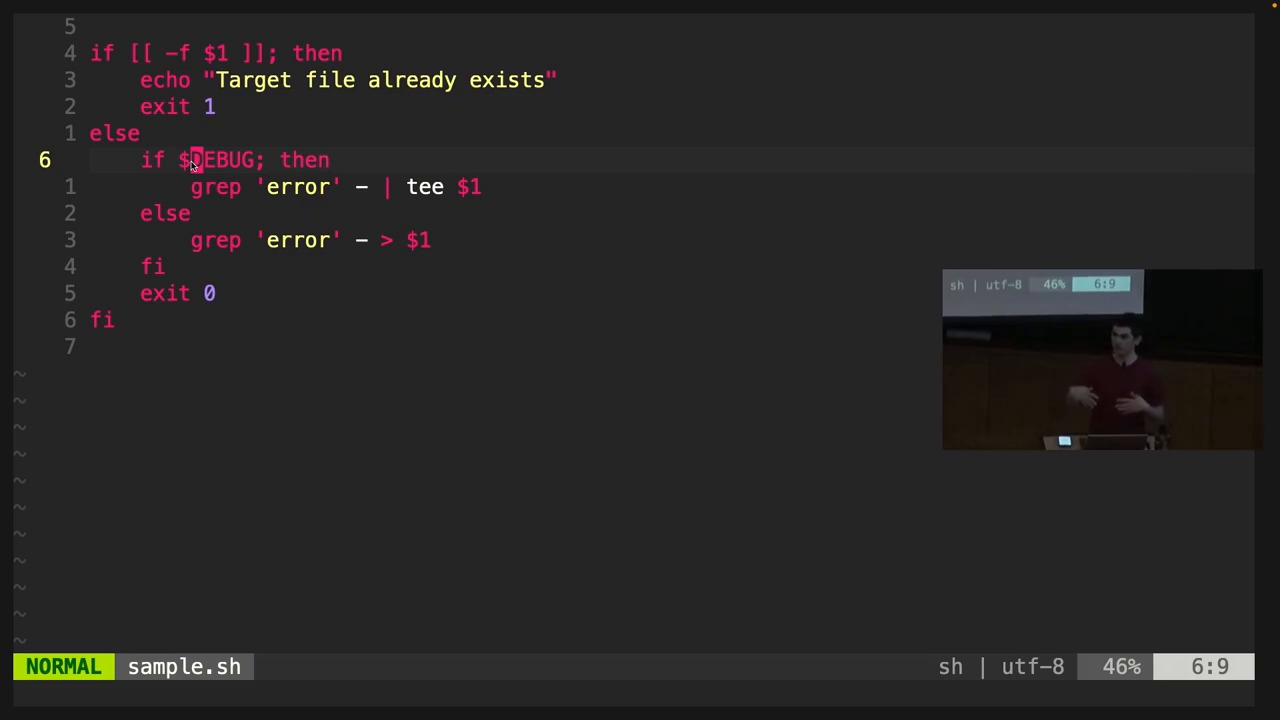
\includegraphics[width=0.92\textwidth]{figures/fig_01_script_overview.jpg}
\caption{讲者开场展示的一段 Shell 脚本，几乎集中了本讲所有概念\vtag}
\end{figure}
\srcnote{00:02:00--00:02:15}
\end{minipage}


讲者先拿 Python 函数作对比：一个函数有参数 $x$ 和 $y$，再返回一个值，输入和输出一目了然。可是读别人的 Shell 脚本时，输入输出往往并不清楚。他展示的脚本里，有的值不知从哪里来，不存在就退出；有的变量并没有在脚本里定义。他说大家现在不必看懂这段脚本，因为它恰好包含了今天要讲的全部概念：Shell 程序有多种输入和多种输出，而且由于程序之间要互相通信、作者又各不相同，几乎所有程序都遵守一套约定。

本讲的路线是：先讲命令行界面的五个概念，即参数、流、环境变量、返回码和信号；再讲远程机器与 SSH、终端复用器 tmux；然后讲怎样定制 Shell，包括包管理器、\texttt{PATH}、配置文件、dotfiles 和插件；最后讲 Shell 中的 AI 工具与终端模拟器。

\begin{importantbox}{一个程序的全部输入和输出}
本讲可以用一张清单来概括。一个命令行程序的输入有三种：命令行参数、标准输入、环境变量；输出有三种：标准输出、标准错误、返回码；此外，程序在运行中还会收到信号。后面每一节都在展开这张清单中的一项，理解了它们，绝大多数陌生的命令都能按同样的规则去使用。
\end{importantbox}

\section{参数与约定}

\subsection{参数就是字符串}

\noindent\begin{minipage}{\textwidth}
\begin{figure}[H]
\centering
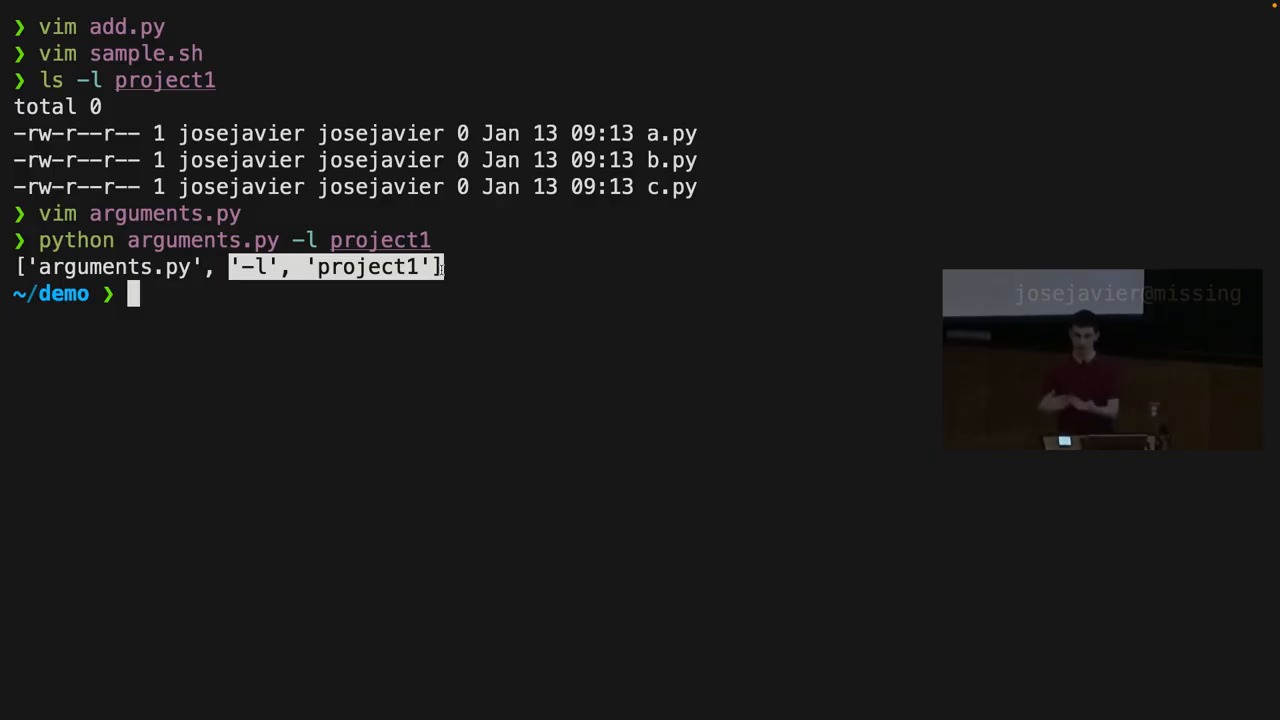
\includegraphics[width=0.92\textwidth]{figures/fig_02_args_python.jpg}
\caption{用一个只打印 \texttt{sys.argv} 的 Python 脚本观察程序收到的参数\vtag}
\end{figure}
\srcnote{00:03:30--00:03:45}
\end{minipage}


最简单的输入就是参数。运行 \texttt{ls -l project1} 时，我们以参数的形式给了程序输入。讲者强调，参数并没有什么特别：\texttt{ls} 拿到的就是字符串 \texttt{-l} 和 \texttt{project1}，再自己解析它们来决定做什么。大多数编程语言都有办法拿到这些信息，在 Python 里是 \texttt{sys.argv}。他写了一个只把收到的参数打印出来的 Python 脚本，用同样的参数运行，可以看到 Shell 调用程序时，程序收到的就是程序名和后面这些参数，如何解释它们完全由程序决定。

\begin{lstlisting}[language=Python]
import sys
print(sys.argv)
\end{lstlisting}

\subsection{选项的约定}

\noindent\begin{minipage}{\textwidth}
\begin{figure}[H]
\centering
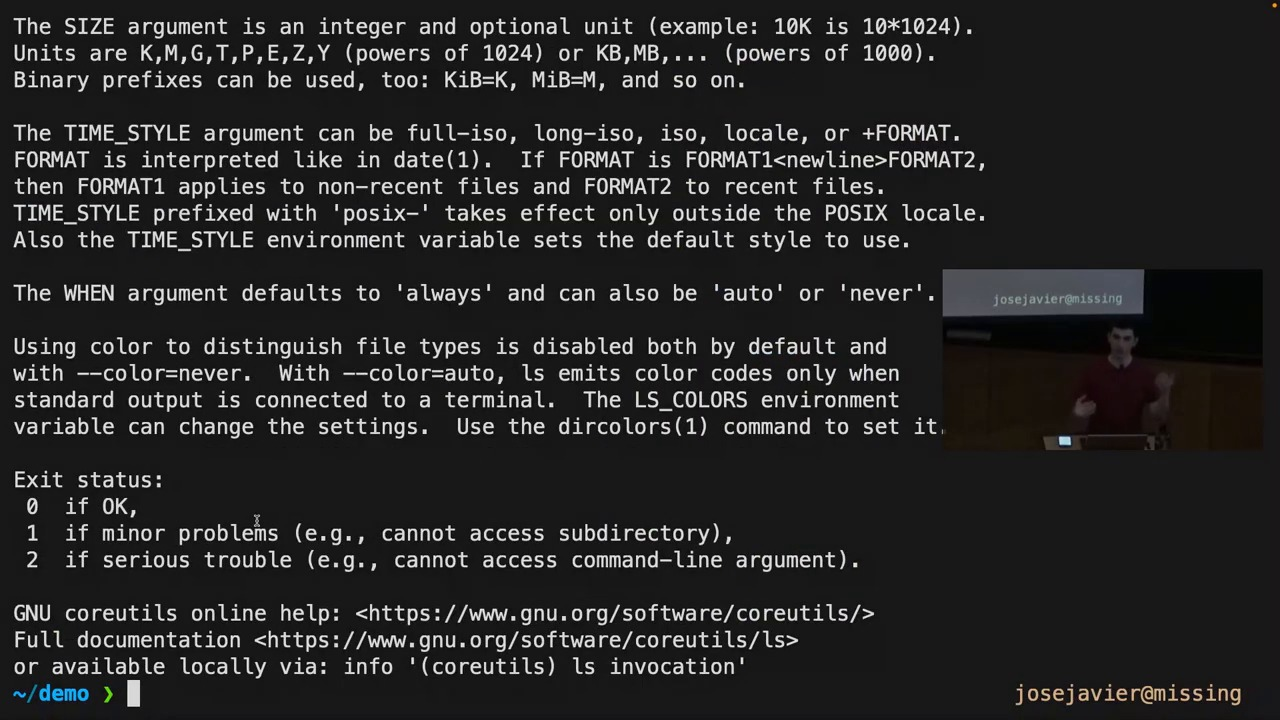
\includegraphics[width=0.92\textwidth]{figures/fig_03_ls_flags.jpg}
\caption{\texttt{ls} 的手册页中记录的大量选项\vtag}
\end{figure}
\srcnote{00:06:00--00:06:15}
\end{minipage}


这里出现了 Shell 里第一个很常见的约定：选项（flag）。带单短横线或双短横线的参数，告诉程序这是一个选项，而不是普通字符串。查看手册页时会看到许多这样的选项。讲者也说明，Shell 并不强制使用这种写法，这是大家约定俗成的，也能找到不遵守它的程序。

进一步的约定是：单短横线后面通常跟一个字母，双短横线后面跟一个完整的单词。例如 \texttt{-a} 表示同时列出隐藏文件，而按约定，隐藏文件就是以点开头的文件。讲者 \texttt{touch} 了一个叫 \texttt{.a} 的文件，直接 \texttt{ls} 看不到它，加上 \texttt{-a} 它就出现了。\texttt{-a} 等价于 \texttt{-{}-all}，可以把前者看作后者的简写。

多个选项通常可以以任意顺序给出，单字母的选项往往还能合并，比如 \texttt{ls -la} 和分开写效果一样。讲者特别指出：这些便利不是 Shell 提供的，而是 \texttt{ls} 程序自己做了解析。所以自己写命令行程序时，通常会用现成的库来自动完成这类解析。另一些常见约定是 \texttt{-h} 或 \texttt{-{}-help} 表示帮助，\texttt{-{}-version} 表示版本。

\begin{knowledgebox}{双短横线 \texttt{-{}-} 的含义}
课程讲义的练习里提到一个特殊参数：单独的 \texttt{-{}-} 告诉程序“后面不要再解析选项了”，之后的一切都当作位置参数。例如要创建或删除一个名字以短横线开头的文件，可以写 \texttt{touch -{}- -myfile}，否则程序会把 \texttt{-myfile} 当成一组选项。
\end{knowledgebox}

\subsection{接受任意多个参数}

另一个常见约定是：程序接受同一类参数任意多次，并对每一个做同样的操作。例如 \texttt{mkdir project3 project4} 一次创建两个目录，而不必分别调用。讲者说这并非一定成立，取决于具体程序，但很多程序都这样设计。这个约定在下一小节的通配符里会显出威力。

\subsection{通配符展开}

\noindent\begin{minipage}{\textwidth}
\begin{figure}[H]
\centering
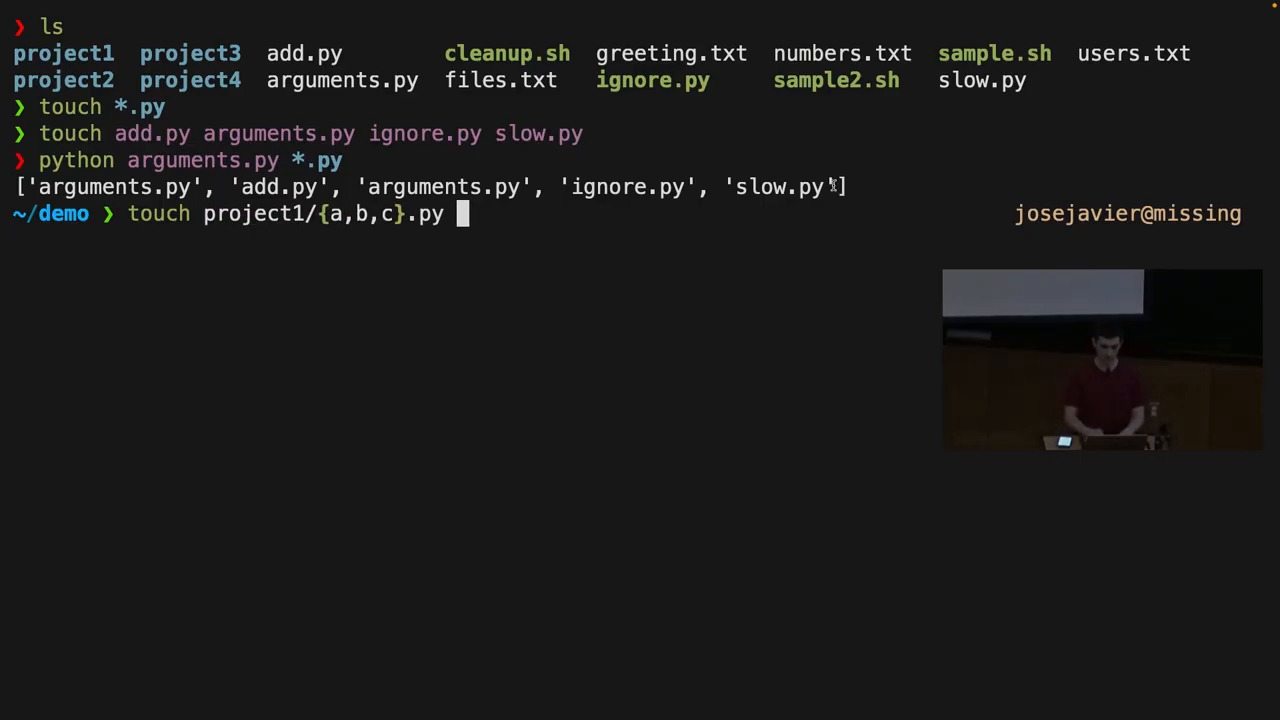
\includegraphics[width=0.92\textwidth]{figures/fig_04_globbing.jpg}
\caption{通配符展开：\texttt{touch *.py} 中的 \texttt{*.py} 在程序运行前就被替换成了文件列表\vtag}
\end{figure}
\srcnote{00:09:00--00:09:15}
\end{minipage}


\texttt{touch} 只是更新文件的修改时间。想更新当前目录下所有 Python 文件，可以写 \texttt{touch *.py}，这是一种叫通配符（globbing）的模式匹配。讲者强调，\texttt{touch} 收到的并不是 \texttt{*.py} 这个字符串，而是 Shell 先把它展开成当前目录中所有匹配的文件名。用前面那个打印参数的 Python 脚本可以验证：传入 \texttt{*.py}，脚本收到的是一串具体的文件名。

通配符是一种很简单的语言，远没有正则表达式强大，但能让很多常见模式写得很简单。例如花括号展开 \texttt{touch \{a,b\}.txt} 会展开成两个文件名；也可以一次匹配 Python 文件和 Shell 脚本。讲者这里用的是 Z shell（zsh），它支持更复杂的通配：\texttt{**/*.py} 中的双星号可以匹配嵌套的子目录，于是能列出整个目录树里的 Python 文件。正因为许多程序接受任意多个参数，通配符才这样好用。

\begin{warningbox}{通配符由 Shell 展开，不是由程序展开}
讲义作者提醒：由于展开发生在程序启动之前，如果没有任何文件匹配，不同 Shell 的行为不同，bash 默认把原样的 \texttt{*.py} 传给程序，zsh 默认直接报错。需要把星号原样交给程序（例如交给 \texttt{find -name}）时，要加引号写成 \texttt{"*.py"}。
\end{warningbox}

\subsection{本章小结}

参数就是字符串，选项、合并短选项、帮助选项都只是约定，由程序自己解析；通配符则由 Shell 在启动程序之前展开。下一节看程序的另一类输入输出：流。

\section{流}

\subsection{管道里的程序同时运行}

\noindent\begin{minipage}{\textwidth}
\begin{figure}[H]
\centering
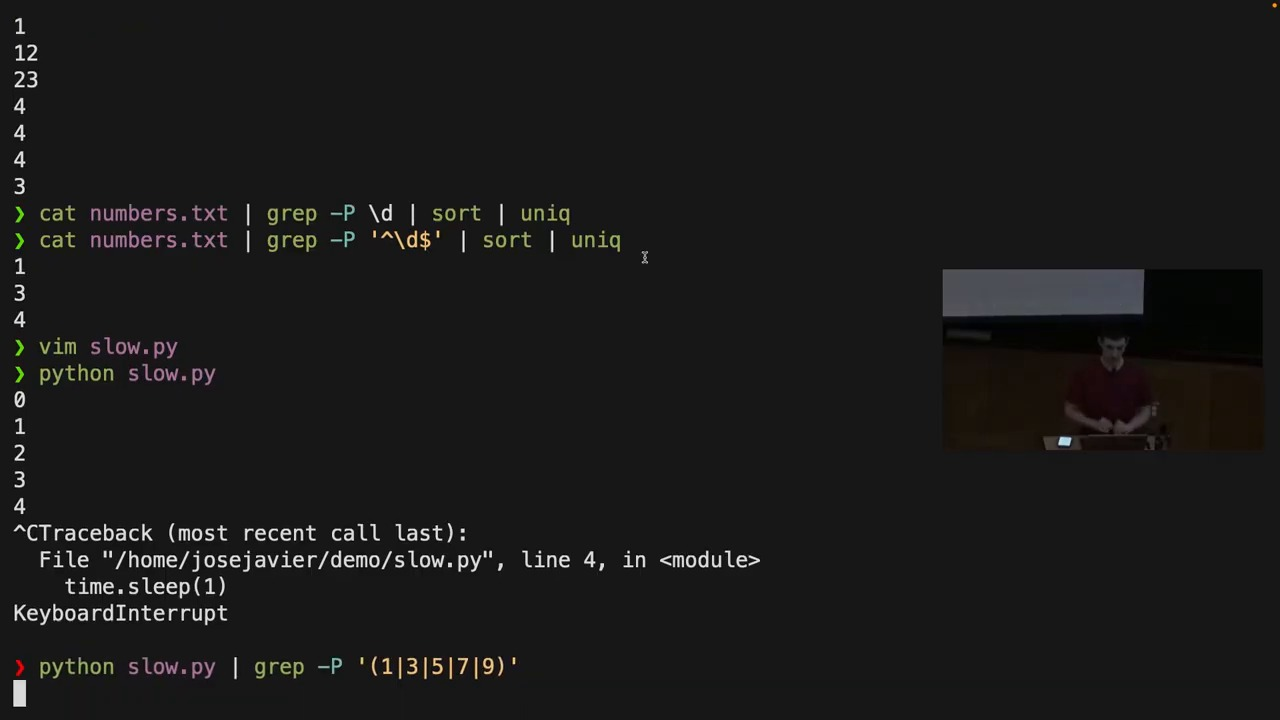
\includegraphics[width=0.92\textwidth]{figures/fig_05_pipeline.jpg}
\caption{管道中的各个程序并行运行，前一个的输出一产生就被后一个消费\vtag}
\end{figure}
\srcnote{00:12:00--00:12:15}
\end{minipage}


上一讲里，我们给程序输入，程序产生输出，再用管道把它们串起来。讲者用一个装着一堆数字的文件演示：\texttt{cat} 出内容，再用 \texttt{grep} 只保留一位数（他发现模式需要加引号）。他强调的要点是：执行管道时，并不是先运行第一个命令、再运行第二个命令，而是所有程序并行运行，前一个程序的输出连接到后一个程序的输入，输出一产生就被下一个进程消费。

他写了一个 Python 脚本，每隔一段时间产生一个数字，后面接一个只保留奇数的过滤器。由于 Python 默认会缓冲输出，需要关闭缓冲才能看清现象：数字一个个产生，两个程序同时在跑，前者生产、后者消费并输出。

\noindent\begin{minipage}{\textwidth}
\begin{figure}[H]
\centering
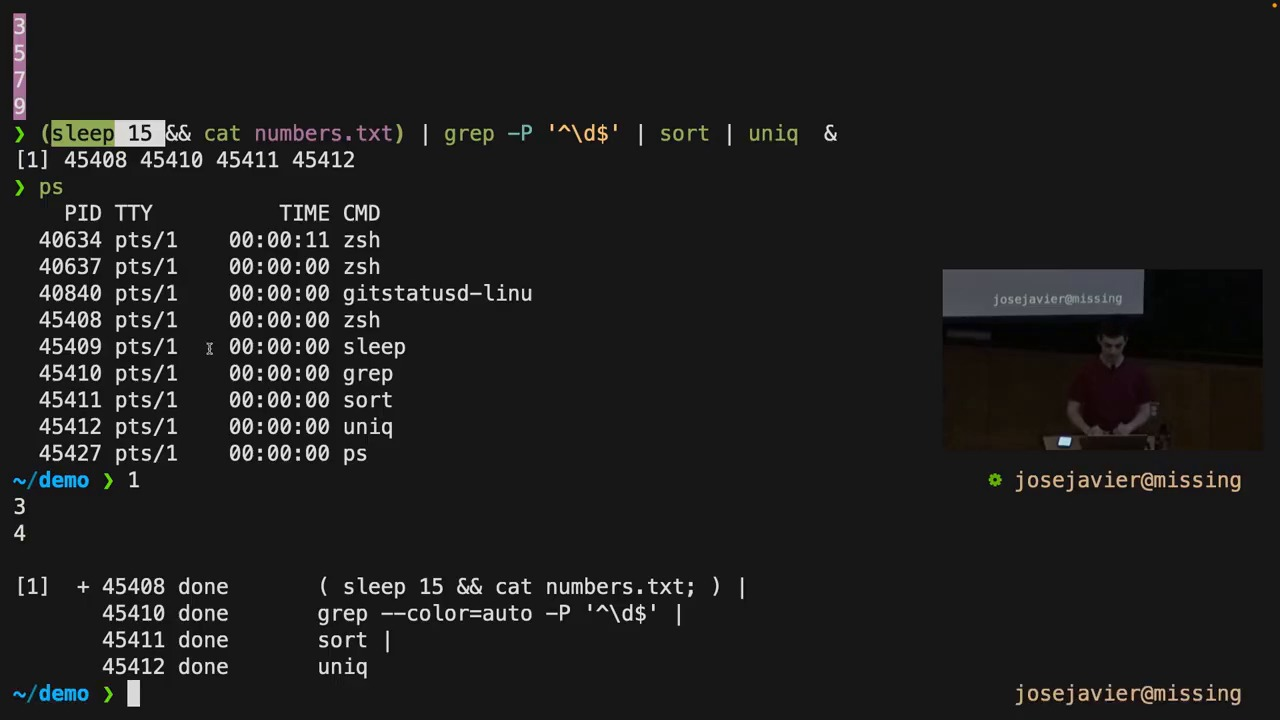
\includegraphics[width=0.92\textwidth]{figures/fig_06_jobs_bg.jpg}
\caption{在后台运行一条管道后用 \texttt{jobs} 和 \texttt{ps} 观察哪些进程已经启动\vtag}
\end{figure}
\srcnote{00:13:00--00:13:15}
\end{minipage}


接着他启动了一条更复杂的管道，形如 \texttt{sleep 15 \&\& cat numbers.txt | sort | uniq \&}，末尾的 \texttt{\&} 把它放到后台。查看进程会发现 \texttt{sleep}、\texttt{sort}、\texttt{uniq} 都已经在了，唯独 \texttt{cat} 不在：因为 \texttt{\&\&} 让 \texttt{cat} 等到 \texttt{sleep} 结束才启动。等一切完成，才得到输出。有同学问能否调整计算机执行这些任务的顺序，讲者解释，这里 \texttt{cat} 之所以没有运行，正是因为用了 \texttt{\&\&}，这是“与”运算符，后面讲返回码时会细说。

\begin{knowledgebox}{缓冲为什么会掩盖并行}
讲义作者补充：许多程序在输出连到管道而不是终端时，会把输出攒成一大块再写出，这叫块缓冲。于是下游看起来像是“等上游跑完才开始”。Python 可以用 \texttt{python -u} 或 \texttt{print(..., flush=True)} 关闭缓冲，\texttt{grep} 有 \texttt{-{}-line-buffered} 选项，这样才能看到逐行流动的效果。
\end{knowledgebox}

\subsection{标准输入}

程序有一个标准输入（stdin），这是它获取信息的方式。大多数程序默认从标准输入读数据，比如 \texttt{grep} 通常就是这样拿到内容的；它也可以直接从文件读，把文件名作为参数即可。还有一个约定：单独的一个短横线 \texttt{-} 表示标准输入。讲者提醒，在这种用法里这个短横线不是选项，而是约定用来表示“从输入读取”。

\subsection{标准输出与标准错误}

\noindent\begin{minipage}{\textwidth}
\begin{figure}[H]
\centering
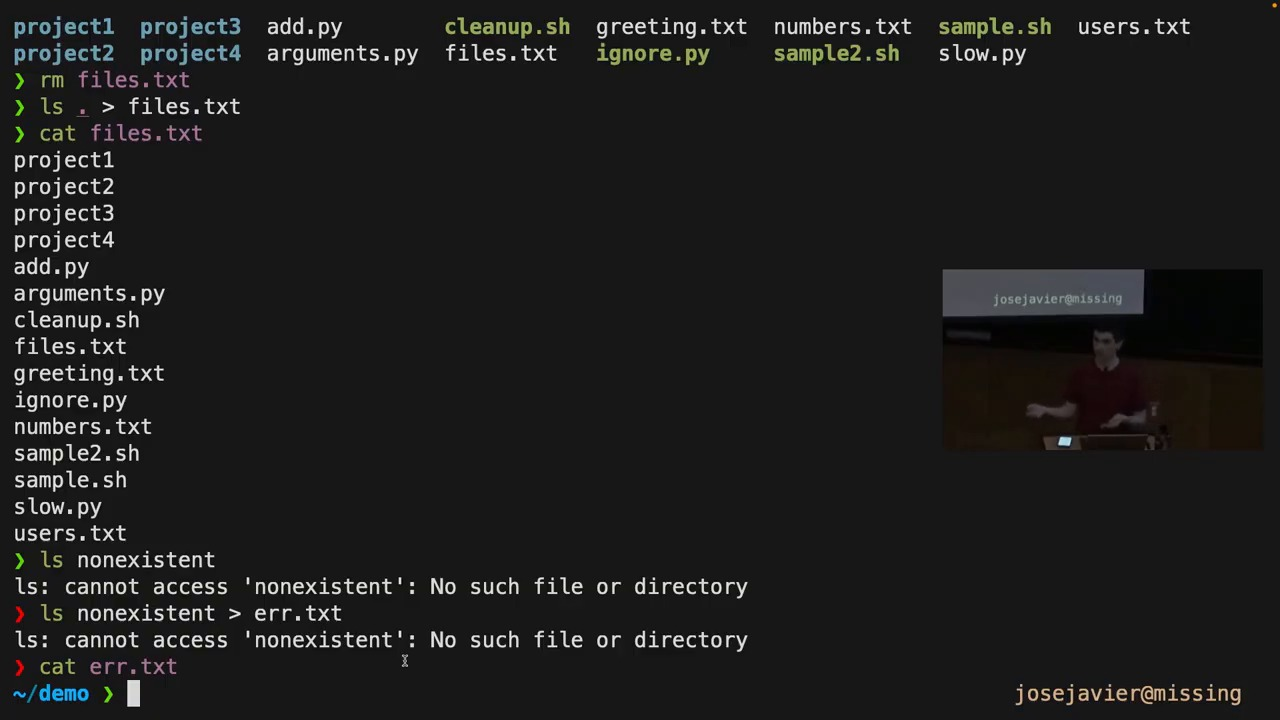
\includegraphics[width=0.92\textwidth]{figures/fig_07_stderr.jpg}
\caption{标准输出被重定向进文件，而错误信息仍然出现在屏幕上\vtag}
\end{figure}
\srcnote{00:15:30--00:15:45}
\end{minipage}


输入只有一个，输出却有两个：标准输出（stdout）和标准错误（stderr）。\texttt{ls} 的列表默认写到标准输出，可以用 \texttt{>} 把它送进 \texttt{files.txt}。但如果 \texttt{ls} 一个不存在的目录，会得到一条错误信息，再用同样的方式去捕获，却发现没有捕获到：它没有进标准输出，而是进了标准错误。要捕获错误需要不同的语法，例如 \texttt{2> err.txt}。讲者说这很方便，因为程序可以分别传递这两类信息，而不会让它们混在一起。

还有一些特殊文件，例如 \texttt{/dev/null}，写进去的东西都会消失，实际上不会写到任何地方。想丢弃不关心的输出时，就把它重定向到这里。

\begin{practicebox}{常用重定向写法}
讲义作者整理：
\begin{itemize}
\item \texttt{cmd > out.txt}：标准输出写入文件（覆盖），\texttt{>>} 表示追加；
\item \texttt{cmd 2> err.txt}：标准错误写入文件，文件描述符 2 就是标准错误；
\item \texttt{cmd > all.txt 2>\&1}：先把标准输出指向文件，再让标准错误跟随它，顺序不能颠倒；
\item \texttt{cmd < in.txt}：用文件内容作为标准输入；
\item \texttt{cmd 2> /dev/null}：丢弃错误信息。
\end{itemize}
\end{practicebox}

\subsection{本章小结}

管道中的程序同时运行，通过标准输入和标准输出相连；错误信息走单独的标准错误，可以单独重定向或丢进 \texttt{/dev/null}。下一节看第三种输入：环境变量。

\section{环境变量}

\subsection{定义与使用变量}

在 bash 里定义变量用 \texttt{foo=bar}，访问用 \texttt{\$foo}。讲者特别强调：\texttt{foo = bar} 这种带空格的写法是不合法的。这样写时，实际上是在让 Shell 运行一个叫 \texttt{foo} 的程序，参数是 \texttt{=} 和 \texttt{bar}，于是 Shell 报告找不到程序 \texttt{foo}，变量也就没有定义。

变量里可以放很多东西，例如用 \texttt{\$(...)} 捕获程序的输出。由于程序通常按换行来切分输入，\texttt{echo} 这个变量会看到内容按行排列；再对它运行 \texttt{grep}，会发现 \texttt{grep} 依然在逐行工作，尽管我们把所有内容放进了一个变量。

\begin{warningbox}{变量要加引号}
讲义作者提醒：\texttt{echo \$var} 和 \texttt{echo "\$var"} 并不一样。不加引号时，变量的值会再被按空白切分并做通配符展开，换行会变成空格，带空格的文件名会被拆成几个参数。讲义中也特意把 \texttt{\$INSTRUCTIONS} 写成带引号的形式。除非确实需要切分，否则引用变量时都应加上双引号。
\end{warningbox}

\subsection{局部变量与 export}

\noindent\begin{minipage}{\textwidth}
\begin{figure}[H]
\centering
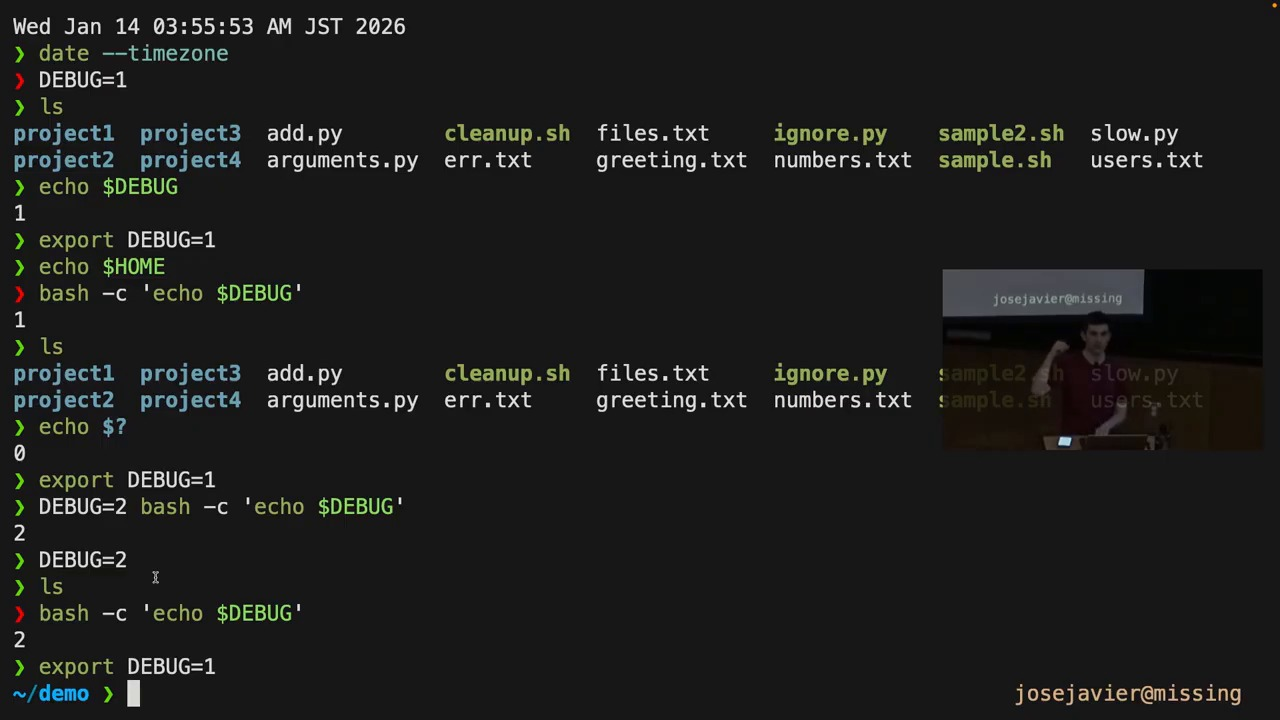
\includegraphics[width=0.92\textwidth]{figures/fig_08_export.jpg}
\caption{只有 \texttt{export} 之后，子进程里的 \texttt{bash -c} 才能看到 \texttt{DEBUG}\vtag}
\end{figure}
\srcnote{00:23:00--00:23:15}
\end{minipage}


有些变量是特殊的。默认情况下，创建的变量只存在于当前的 Shell 会话里，但有时需要把变量传给启动的其他程序。讲者设置 \texttt{DEBUG=1}，再运行一个程序，它启动一个子 Shell 并检查 \texttt{DEBUG} 的值，结果什么也没有：变量只在本地 Shell 里设置了。

有两种办法把它传给子进程。一是在命令前面直接加上赋值，形如 \texttt{DEBUG=1 bash -c 'echo \$DEBUG'}，这样只有这一次启动的程序的环境里有这个变量。二是 \texttt{export DEBUG=1}，告诉 Shell：此后创建的所有子进程都应该得到这个变量。讲者解释，在当前会话里用 \texttt{less} 之类再回来，\texttt{DEBUG} 依然是 $1$，但不 \texttt{export} 的话子进程不会继承它。

有同学问 \texttt{bash -c} 是做什么的：它启动一个 bash，运行右边给出的命令，是创建子 Shell 的一种方式。也有同学问 \texttt{export} 之后再修改变量，子 Shell 里是否也会变：讲者的回答是会，因为已经声明它是导出的，之后启动的子进程拿到的是新值。

\begin{knowledgebox}{子进程拿到的是副本}
讲义作者补充：环境变量在进程启动时被复制给子进程，此后父子双方互不影响。所以子进程修改环境变量不会改变父 Shell；“修改后子 Shell 也会变”只对修改之后才启动的子进程成立，已经在运行的子进程看不到变化。
\end{knowledgebox}

\subsection{约定俗成的环境变量}

\noindent\begin{minipage}{\textwidth}
\begin{figure}[H]
\centering
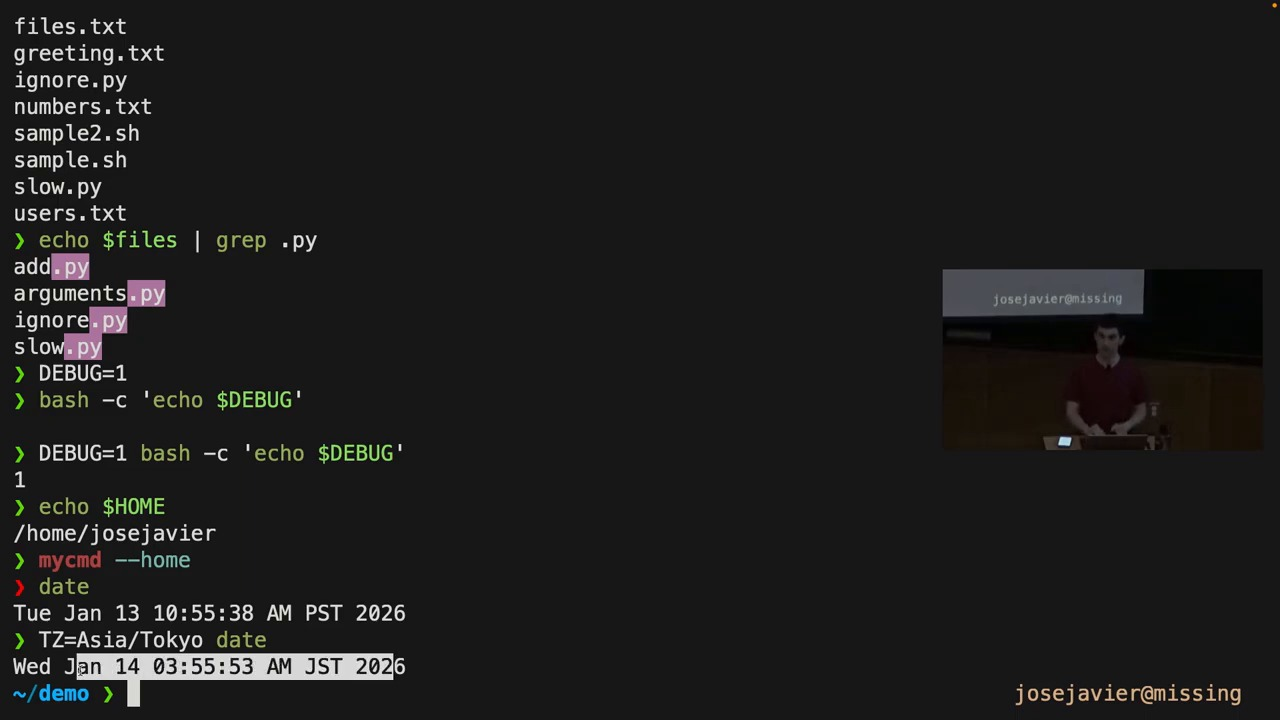
\includegraphics[width=0.92\textwidth]{figures/fig_09_tz_date.jpg}
\caption{设置 \texttt{TZ=Asia/Tokyo} 后，\texttt{date} 的输出随之改变\vtag}
\end{figure}
\srcnote{00:19:30--00:19:45}
\end{minipage}


环境变量之所以有用，是因为有些变量的用法是约定好的。例如程序想保存配置时，可能会查看 \texttt{HOME} 环境变量，知道“这个用户的主目录在这里”，而不必每次都由用户指定。另一个例子是上一讲见过的 \texttt{date}：设置 \texttt{TZ} 环境变量为 \texttt{Asia/Tokyo} 再运行，输出就变了，因为 \texttt{date} 会检查这个变量并据此改变行为。讲者说时区这类信息很多程序都需要，用环境变量统一传递就很方便。

\subsection{本章小结}

变量赋值不能有空格；普通变量只在当前 Shell 有效，\texttt{export} 或命令前缀赋值才能传给子进程；\texttt{HOME}、\texttt{TZ} 等约定变量让程序无需额外参数就能得到上下文。下一节看程序的第三种输出：返回码。

\section{返回码}

\noindent\begin{minipage}{\textwidth}
\begin{figure}[H]
\centering
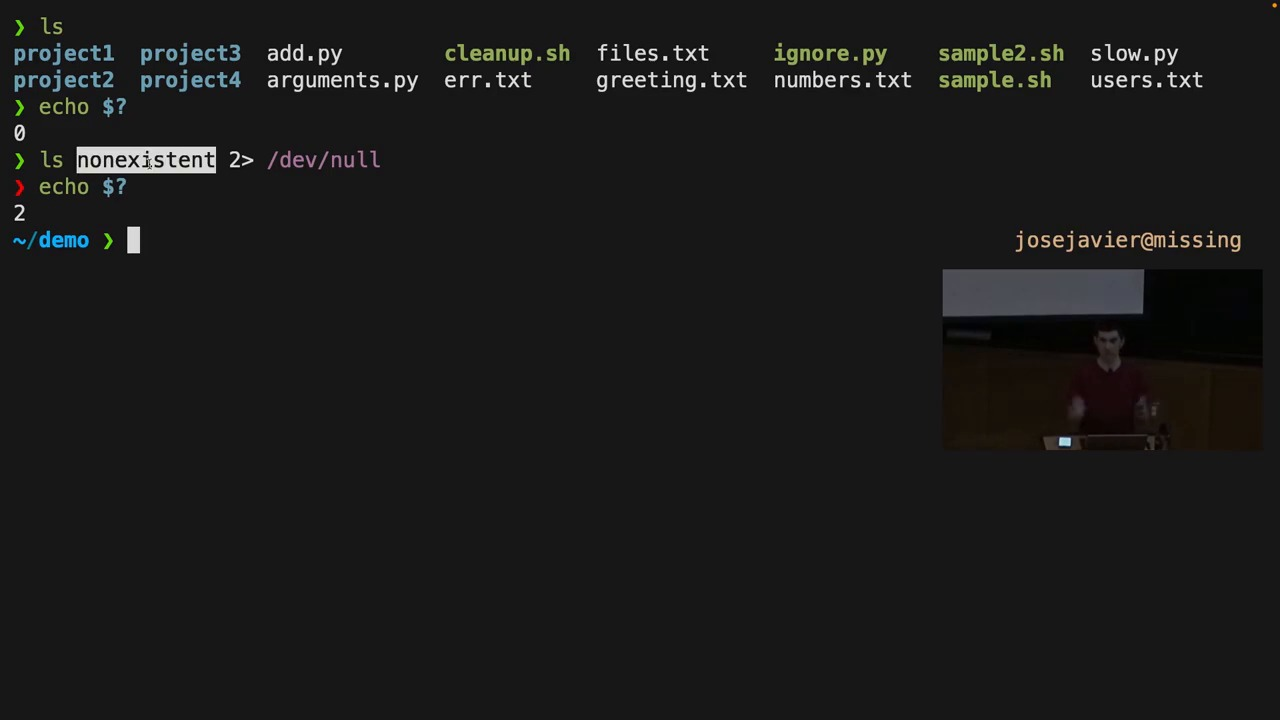
\includegraphics[width=0.92\textwidth]{figures/fig_10_return_code.jpg}
\caption{用 \texttt{echo \$?} 查看上一条命令的返回码\vtag}
\end{figure}
\srcnote{00:24:15--00:24:30}
\end{minipage}


我们已经看到，程序通过参数、环境变量和标准输入获得输入，通过标准输出产生输出。还有一种输出是返回码（return code）。标准输出可以看作一串字符串，但很多时候需要表明命令是否成功。运行 \texttt{ls} 一切正常时，可以用 \texttt{echo \$?} 查看返回码，它也是一个以字符串表示的数字，这里是 $0$。约定是：$0$ 表示成功，非零表示出了问题。\texttt{ls} 一个不存在的目录，返回码就是非零。

讲者强调，Shell 语言中的大多数运算符依赖的是返回码。上一讲见到的 \texttt{if}、\texttt{while} 等几乎所有控制流，看的都不是程序的输出，而是它的返回码。

\noindent\begin{minipage}{\textwidth}
\begin{figure}[H]
\centering
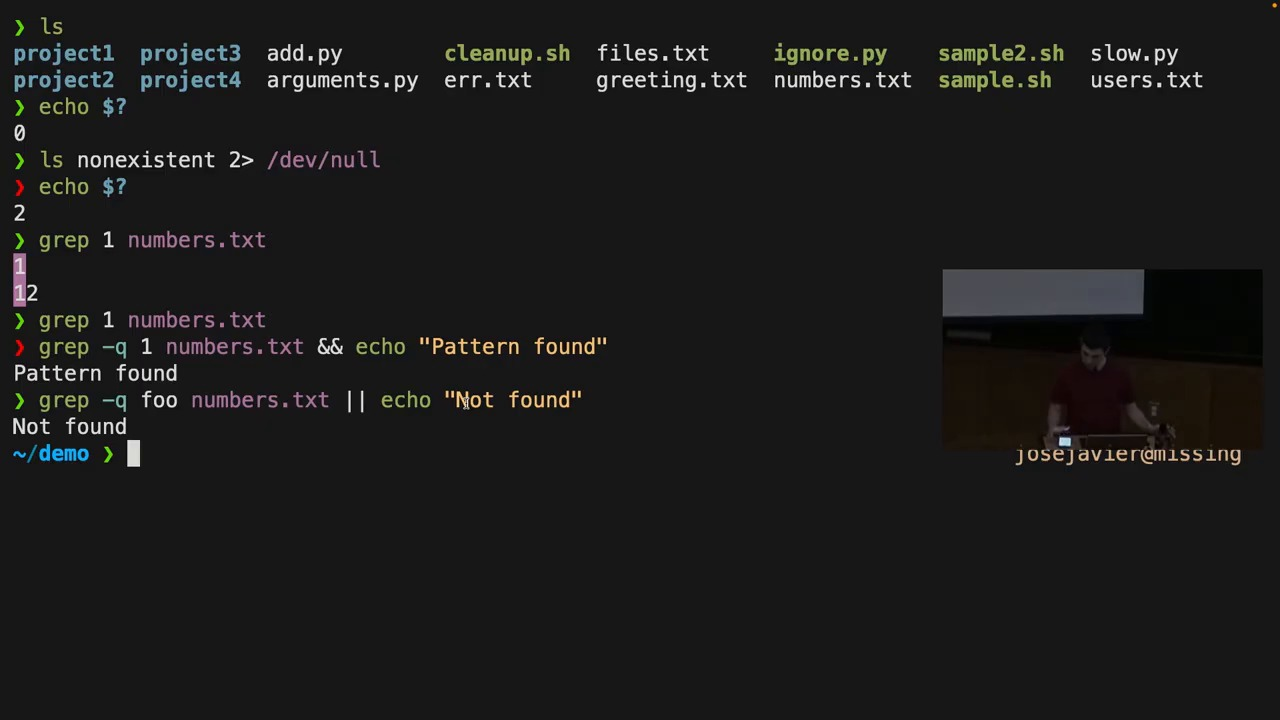
\includegraphics[width=0.92\textwidth]{figures/fig_11_grep_q.jpg}
\caption{\texttt{grep -q} 不输出任何内容，只用返回码告诉后面的命令是否找到\vtag}
\end{figure}
\srcnote{00:25:30--00:25:45}
\end{minipage}


例如 \texttt{grep} 找到匹配时返回 $0$，找不到时返回非零。配合 \texttt{\&\&}（与）运算符，第二个程序只有在第一个成功时才运行；反过来，\texttt{||}（或）运算符让第二个命令只在前一个失败时才运行。讲者演示了 \texttt{grep -q 1 numbers.txt \&\& echo "Pattern found"} 以及对应的 \texttt{||} 版本。有同学问 \texttt{-q} 是什么：它等价于“安静”，只尝试匹配、不产生任何输出。这样做的原因是我们只想用 \texttt{grep} 的返回码。

\begin{lstlisting}[language=bash]
grep -q 1 numbers.txt && echo "Pattern found"
grep -q 7 numbers.txt || echo "Not found"
\end{lstlisting}

\begin{knowledgebox}{管道的返回码}
讲义作者补充：一条管道的返回码默认是最后一个命令的返回码，前面的命令失败会被“吞掉”。在 bash 中执行 \texttt{set -o pipefail} 之后，只要管道中有一个命令失败，整条管道就返回非零，写脚本时常与 \texttt{set -e} 一起使用。
\end{knowledgebox}

\subsection{本章小结}

返回码是程序报告成败的方式，$0$ 为成功；\texttt{if}、\texttt{while}、\texttt{\&\&}、\texttt{||} 都依据它工作，\texttt{grep -q} 这类选项就是专门为“只要返回码”的场景设计的。最后一个 Shell 概念是信号。

\section{信号与任务控制}

\subsection{信号是软件中断}

\noindent\begin{minipage}{\textwidth}
\begin{figure}[H]
\centering
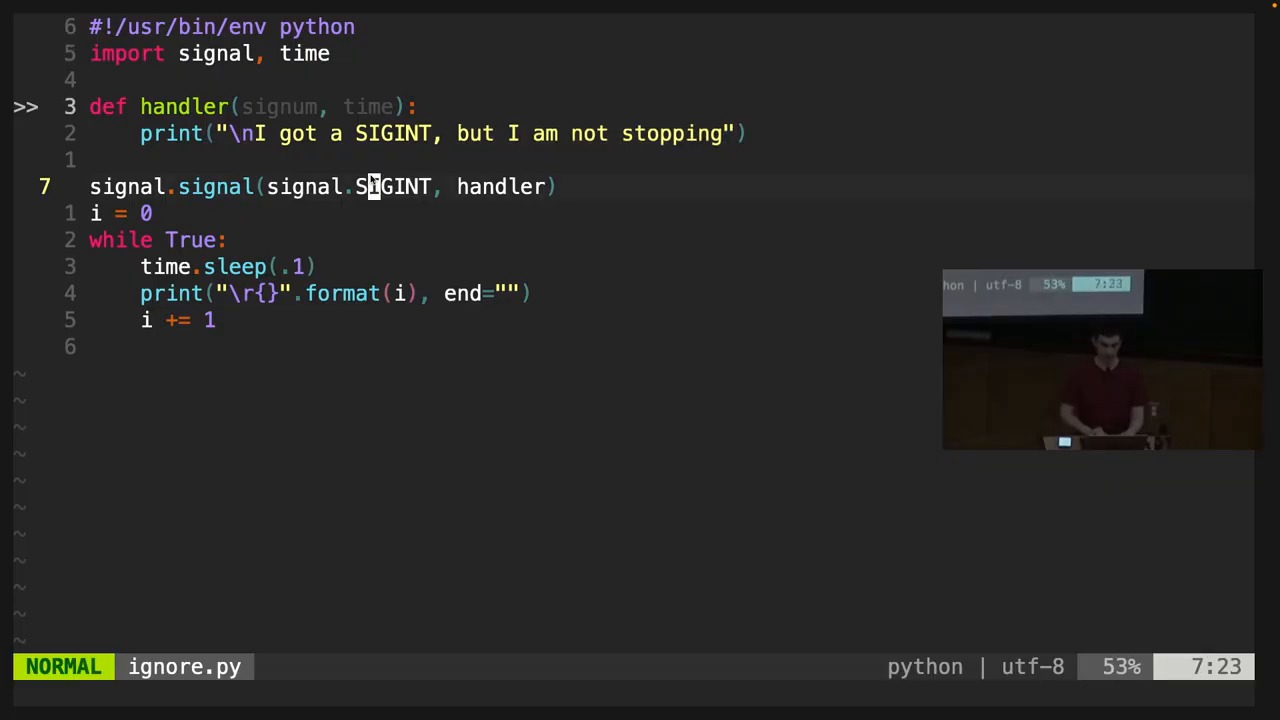
\includegraphics[width=0.92\textwidth]{figures/fig_12_sigint_handler.jpg}
\caption{一个捕获 \texttt{SIGINT} 并拒绝退出的 Python 程序\vtag}
\end{figure}
\srcnote{00:27:15--00:27:30}
\end{minipage}


上一讲看到，按 Ctrl+C 可以让一个运行中的命令停下来。背后发生的事情是：Shell 给程序发送了信号（signal）。信号是一种软件中断，Shell 发送带有特定编号的信号，程序收到后，如果有处理它的代码就执行那段代码，否则多半直接退出。

讲者用 Python 的 \texttt{signal} 库定义了一个处理函数，它打印“收到 SIGINT，但我不打算停”，并注册为 \texttt{SIGINT} 的处理函数；主循环只是不断数数。运行后按 Ctrl+C，程序并不停止，因为我们自己处理了这个信号并决定忽略它。还有更多信号，例如 Ctrl+\textbackslash{} 发送 \texttt{SIGQUIT}，是一种更强硬的“你真的应该退出了”。

\begin{lstlisting}[language=Python]
import signal, time

def handler(signum, time):
    print("\nI got a SIGINT, but I am not stopping")

signal.signal(signal.SIGINT, handler)
i = 0
while True:
    time.sleep(.1)
    print("\r{}".format(i), end="")
    i += 1
\end{lstlisting}

\begin{warningbox}{处理函数的参数名遮蔽了模块}
讲义作者提醒：上面这段与课程讲义一致的代码里，处理函数的第二个参数被命名为 \texttt{time}，在函数内部它会遮蔽同名的 \texttt{time} 模块。这里函数体没有用到 \texttt{time} 模块所以能运行，但通常应命名为 \texttt{frame}，以免在处理函数里调用 \texttt{time.sleep} 时出错。
\end{warningbox}

\subsection{用信号清理临时文件}

\noindent\begin{minipage}{\textwidth}
\begin{figure}[H]
\centering
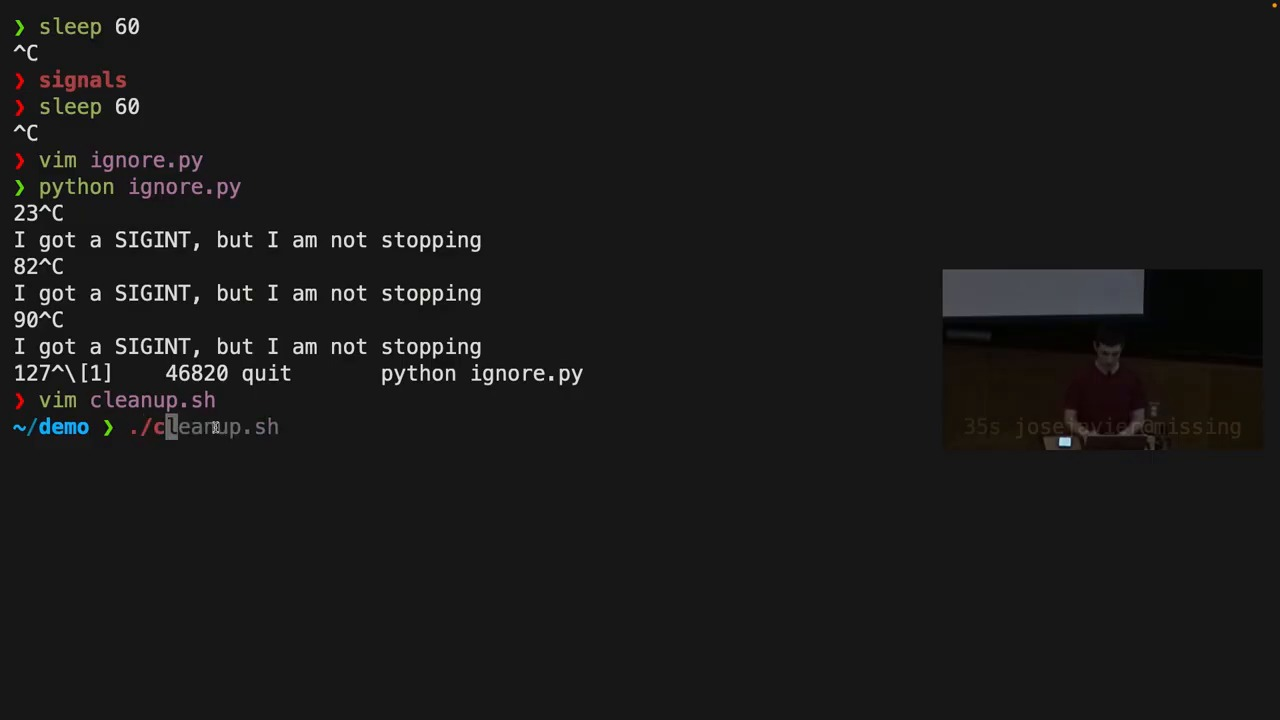
\includegraphics[width=0.92\textwidth]{figures/fig_13_trap_cleanup.jpg}
\caption{收到中断信号时先清理临时文件再退出的脚本\vtag}
\end{figure}
\srcnote{00:28:45--00:29:00}
\end{minipage}


信号定义了很多种，但实践中常用的只有几个。讲者举了一个有用的场景：脚本使用了一些临时文件，希望即使中途出错或被人中断，也能把它们清理掉，不留垃圾。他写了一个 bash 函数负责清理临时文件，并在收到 \texttt{SIGINT} 或 \texttt{SIGTERM} 时调用它；脚本主体是创建文件、睡眠、再删除。运行后按 Ctrl+C，会看到清理信息被打印出来。

\begin{lstlisting}[language=bash]
cleanup() {
    echo "Cleaning up temporary files..."
    rm -f /tmp/mytemp.*
    exit
}
trap cleanup SIGINT SIGTERM
touch /tmp/mytemp.$$
sleep 60
rm -f /tmp/mytemp.$$
\end{lstlisting}

有同学问程序被中断时会不会清理缓存。讲者回答这取决于程序：像这个脚本一样有处理中断的方式，就能清理；默认情况下，如果程序没有处理信号，它不会做任何清理。

\subsection{挂起、继续与 kill}

\noindent\begin{minipage}{\textwidth}
\begin{figure}[H]
\centering
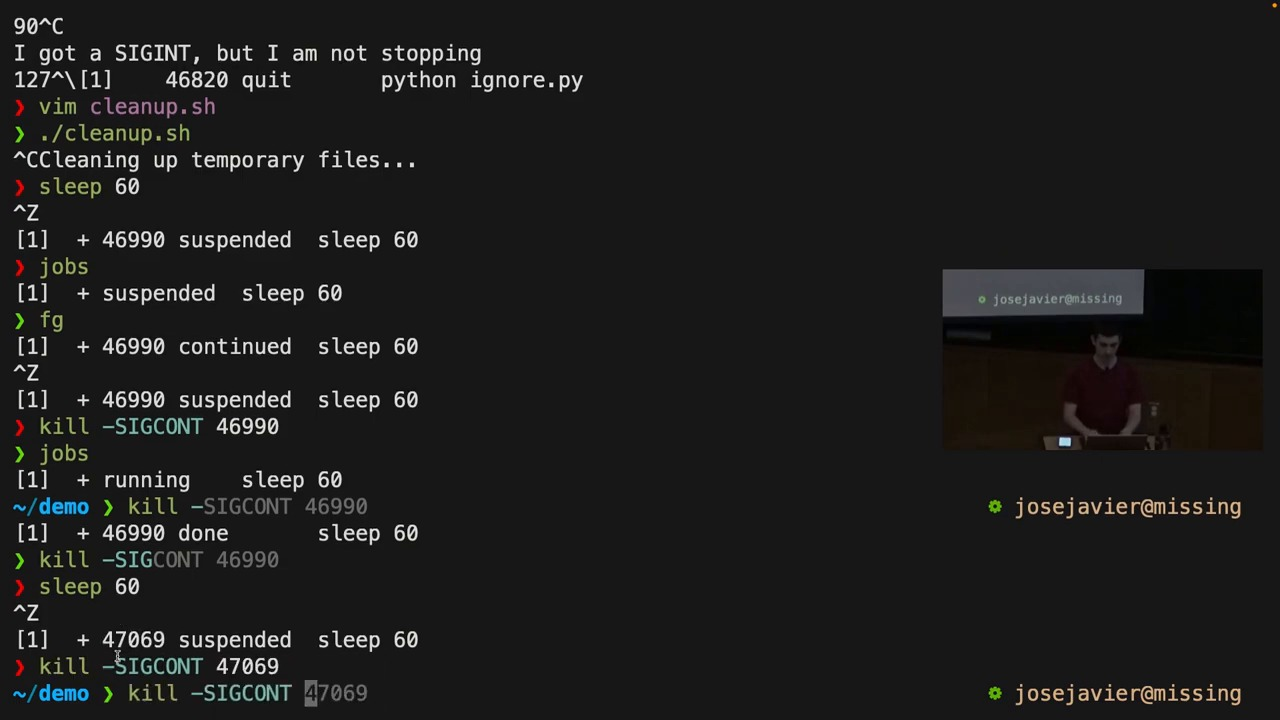
\includegraphics[width=0.92\textwidth]{figures/fig_14_suspend_kill.jpg}
\caption{Ctrl+Z 挂起的进程可以用 \texttt{kill} 发送继续或中断信号\vtag}
\end{figure}
\srcnote{00:30:15--00:30:30}
\end{minipage}


并非所有信号都会终止程序。另一个常见的是 Ctrl+Z：Shell 发送 \texttt{SIGTSTP}，意思是“终端让你暂停”，程序就被挂起。查看进程会看到这个被挂起的进程，可以把它恢复。也可以用 \texttt{kill} 命令给进程发信号：讲者说 \texttt{kill} 只是一种发送任意信号的方式，并不只是用来停止程序。例如向挂起的进程发送继续信号 \texttt{SIGCONT}，它就从挂起变为运行；挂起状态的进程无法用 Ctrl+C 中断，但可以用 \texttt{kill -SIGINT} 显式地发送中断信号。

讲者总结 Shell 的这一部分：选项、从标准输入读、接受参数、接受任意多个参数并对每个执行操作……这些约定随处可见。越多地在日常中使用 Shell，越会发现新程序很容易上手，因为大多数程序都遵守同样的规则。

\begin{practicebox}{任务控制速查}
讲义作者整理：Ctrl+C 发送 \texttt{SIGINT}；Ctrl+\textbackslash{} 发送 \texttt{SIGQUIT}；Ctrl+Z 发送 \texttt{SIGTSTP} 挂起；\texttt{jobs} 列出当前 Shell 的任务；\texttt{fg} 和 \texttt{bg} 让挂起的任务在前台或后台继续；\texttt{kill -STOP} 和 \texttt{kill -CONT} 手动暂停与继续；\texttt{SIGKILL} 无法被捕获，只在程序不响应时使用。
\end{practicebox}

\subsection{本章小结}

信号是 Shell 与运行中程序沟通的方式：程序可以捕获并自定义处理，也可以借此清理资源；挂起与继续同样通过信号完成，\texttt{kill} 能发送任意信号。到这里，命令行界面的五个概念就讲完了，接下来离开本机，去远程机器上工作。

\section{远程机器与 SSH}

\subsection{登录远程 Shell}

\noindent\begin{minipage}{\textwidth}
\begin{figure}[H]
\centering
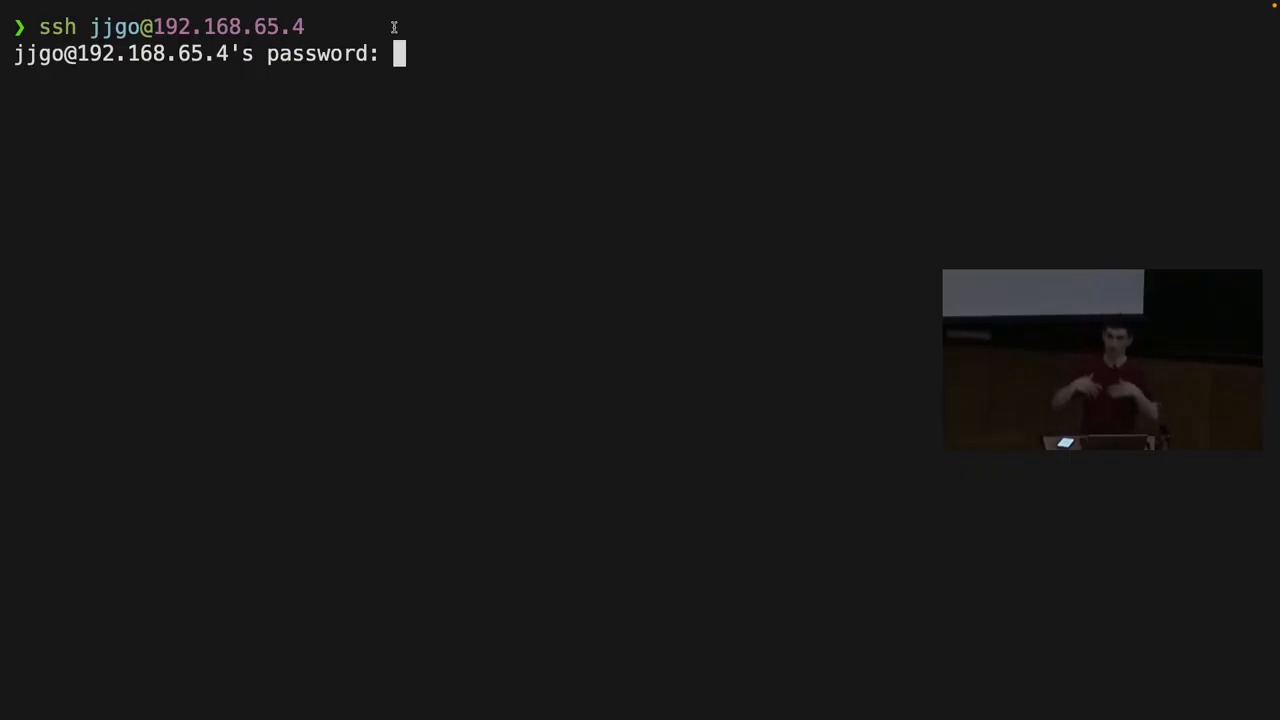
\includegraphics[width=0.92\textwidth]{figures/fig_15_ssh_login.jpg}
\caption{用 \texttt{ssh} 以用户 \texttt{jjgo} 登录一台远程服务器\vtag}
\end{figure}
\srcnote{00:32:45--00:33:00}
\end{minipage}


下一个主题是在不属于自己电脑、而是运行在远程服务器上的 Shell 里工作，用的是安全 Shell（secure shell，SSH）。语法形如 \texttt{ssh jjgo@192.168.65.4}：以用户 \texttt{jjgo} 认证，后面是 IP 地址。讲者解释，IP 地址是更底层的方式，平时常见的是 \texttt{foobar.mit.edu} 这样的域名，实际上计算机会在网上查询，得知它对应哪个数字地址。SSH 通常会提示输入密码，登录后就能像在本地一样创建文件、做几乎所有事。

\subsection{SSH 密钥}

\noindent\begin{minipage}{\textwidth}
\begin{figure}[H]
\centering
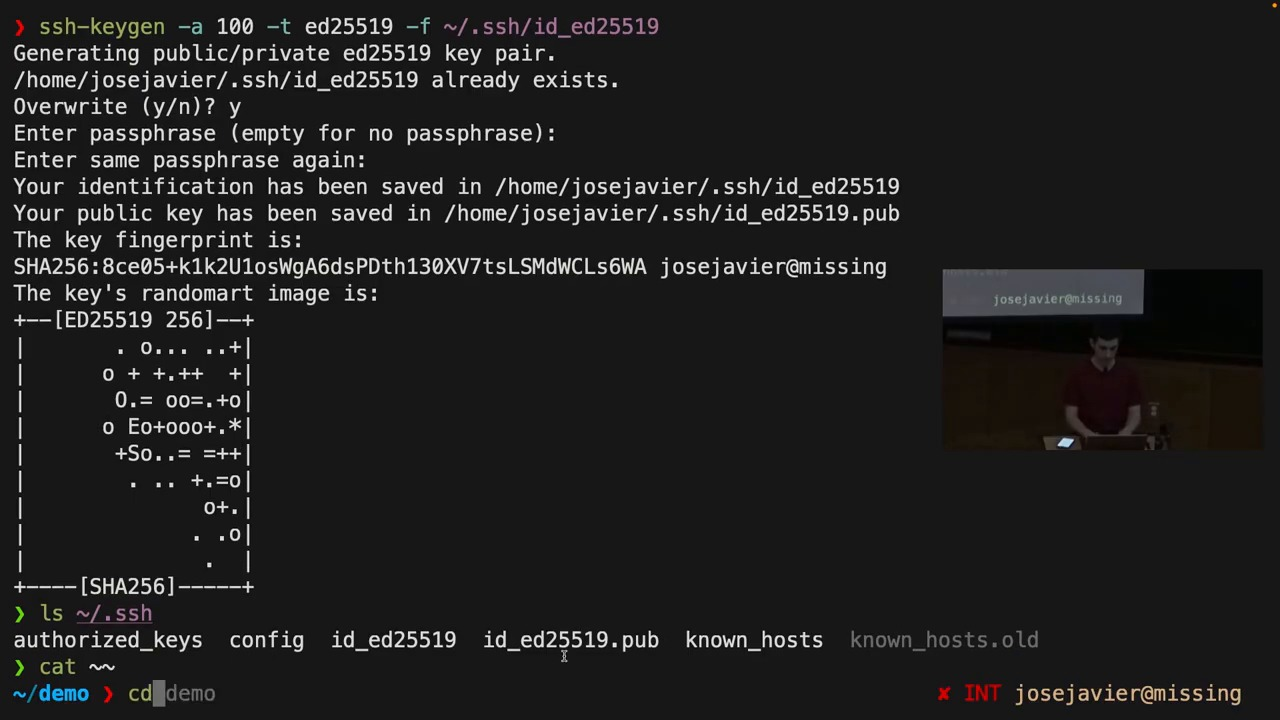
\includegraphics[width=0.92\textwidth]{figures/fig_16_ssh_keygen.jpg}
\caption{\texttt{ssh-keygen} 生成的一对私钥与公钥文件\vtag}
\end{figure}
\srcnote{00:33:45--00:34:00}
\end{minipage}


一件烦人的事是每次退出再登录都要重新认证。为此我们依靠 SSH 密钥。SSH 密钥使用公钥密码学，有一把私钥和一把公钥，借此可以证明自己有权登录而无需输入密码。生成密钥运行 \texttt{ssh-keygen} 一类的命令，之后在 \texttt{\textasciitilde/.ssh} 下会出现两个文件：私钥和公钥。

公钥是可以公开的一段信息：把它放到远程服务器上，服务器就能验证我们确实持有对应的私钥。比如往 GitHub 上传代码时，为了让 GitHub 知道你是谁，你会把公钥给它，它用公钥验证你。私钥则绝不能交给任何人，它不应离开你的电脑，相当于你的密码。讲者说他在课上把密钥显示出来没有关系，因为那只是为课程临时生成的，但大家永远不要把私钥粘贴到任何地方。

\noindent\begin{minipage}{\textwidth}
\begin{figure}[H]
\centering
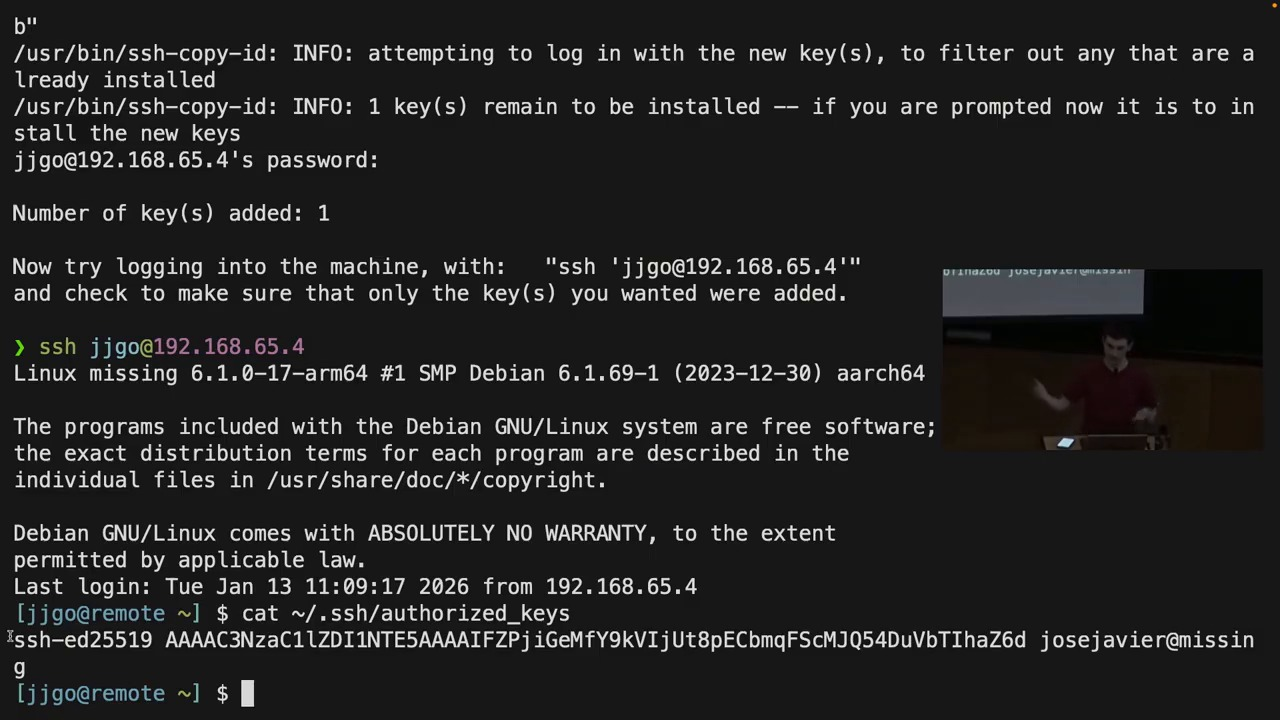
\includegraphics[width=0.92\textwidth]{figures/fig_17_ssh_copy_id.jpg}
\caption{\texttt{ssh-copy-id} 所做的只是把公钥追加进服务器的 \texttt{authorized\_keys}\vtag}
\end{figure}
\srcnote{00:35:00--00:35:15}
\end{minipage}


要让服务器知道我们的公钥，可以用 \texttt{ssh-copy-id}。讲者查看了服务器上 \texttt{.ssh} 目录中的 \texttt{authorized\_keys} 文件，说明这个看似神奇的命令唯一做的事，就是把一个字符串复制过去，让服务器能够验证我们持有私钥。

有同学问创建 SSH 密钥时是否应该设置口令（passphrase）。讲者说应该设：如果不设，相当于把登录这些服务器的密码直接放在文件系统里，任何能读你文件系统的程序大概都能读到它。设置口令后，私钥会用你的口令加密，每次 SSH 登录时会提示你解密。讲义里有一些让这件事更方便的程序的例子。

\begin{warningbox}{私钥与口令}
讲义作者提醒：私钥文件的权限应只允许自己读写（\texttt{chmod 600}），否则 \texttt{ssh} 会拒绝使用；为私钥设置口令后，可以用 \texttt{ssh-agent} 在一次登录会话中只输入一次口令。千万不要把私钥提交进代码仓库或发给他人。
\end{warningbox}

\subsection{远程执行命令与拷贝文件}

\noindent\begin{minipage}{\textwidth}
\begin{figure}[H]
\centering
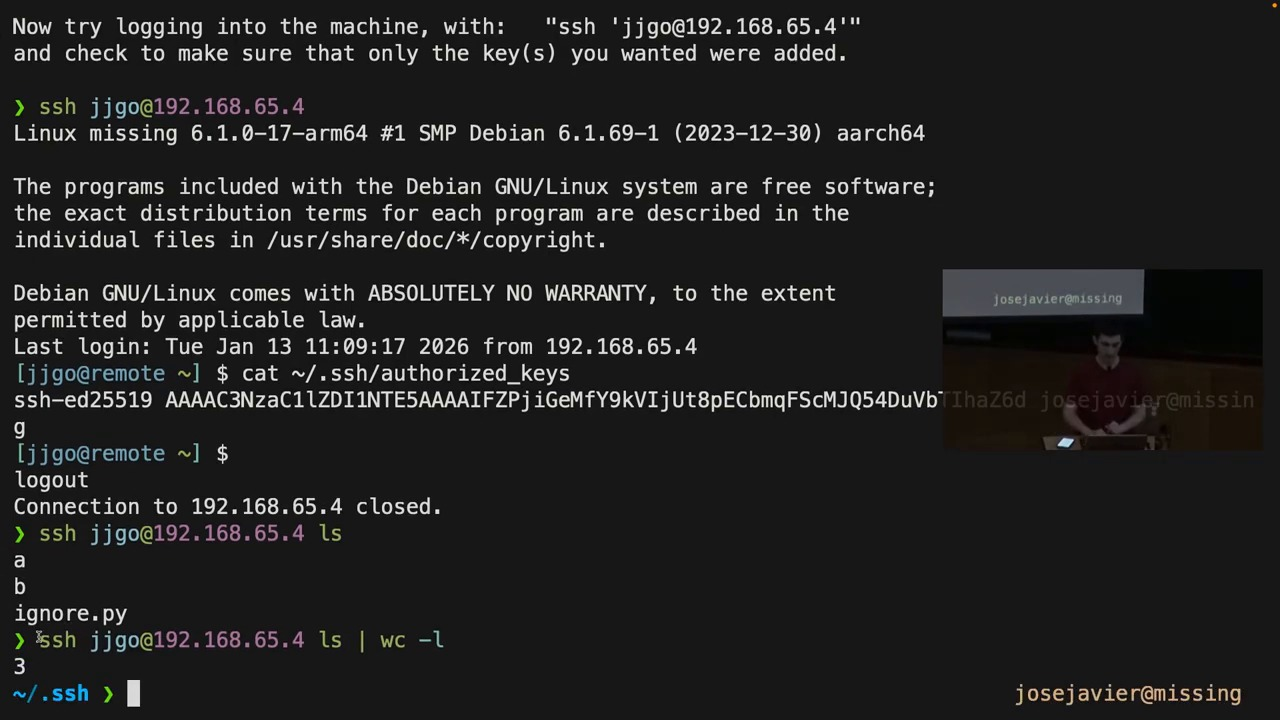
\includegraphics[width=0.92\textwidth]{figures/fig_18_ssh_command.jpg}
\caption{\texttt{ssh} 后面直接跟命令，远程执行的输出被转发回本地\vtag}
\end{figure}
\srcnote{00:35:45--00:36:00}
\end{minipage}


SSH 不只能用于交互式会话，也能执行命令。\texttt{ssh} 后面跟上 \texttt{ls}，就在远程机器上执行 \texttt{ls}，输出被转发为 \texttt{ssh} 自己的输出。讲者说 SSH 并不神奇，它和几乎所有命令一样，接收输入、产生输出。例如 \texttt{ssh server ls | wc -l} 中，\texttt{ls} 在远程运行，而统计行数的 \texttt{wc -l} 在本地运行；如果希望整条管道都在远程执行，就把管道放进引号里交给 \texttt{ssh}。

\noindent\begin{minipage}{\textwidth}
\begin{figure}[H]
\centering
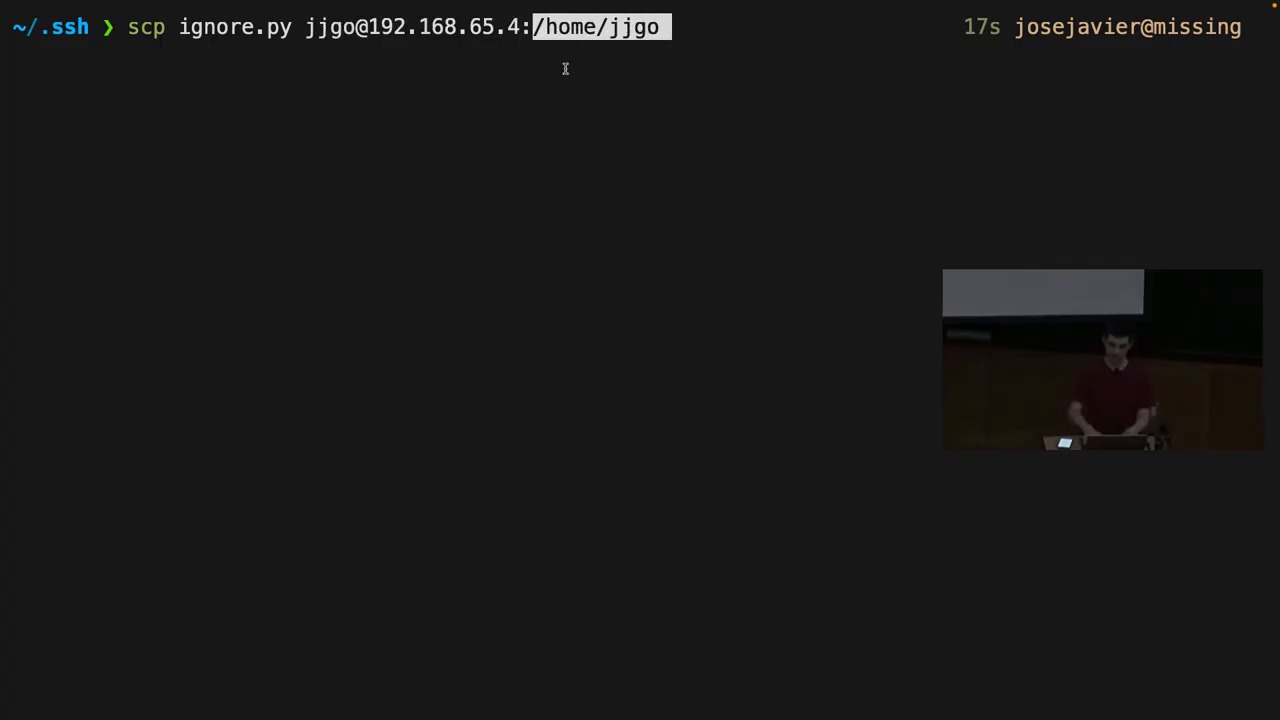
\includegraphics[width=0.92\textwidth]{figures/fig_19_scp.jpg}
\caption{用 \texttt{scp} 把本地文件复制到远程服务器的指定路径\vtag}
\end{figure}
\srcnote{00:37:00--00:37:15}
\end{minipage}


要把本地文件复制到远程机器，有很多程序可用，讲者演示的是 \texttt{scp}：按照它特有的语法写出“本地文件 远程主机:路径”，它会报告复制成功，登录上去就能看到文件已经在那里了。

\begin{knowledgebox}{rsync}
讲义作者补充：拷贝大量文件或需要反复同步时，\texttt{rsync} 通常比 \texttt{scp} 更合适：它只传输有变化的部分，中断后可以续传，常用写法是 \texttt{rsync -avP src/ host:dst/}。
\end{knowledgebox}

\subsection{本章小结}

SSH 让我们在远程机器上获得一个 Shell，密钥省去了反复输入密码，而 SSH 本身也是一个普通的“输入—输出”程序，可以放进管道里。下一个问题是：在远程机器上怎样同时做好几件事，并且不怕断线。

\section{终端复用器 tmux}

\noindent\begin{minipage}{\textwidth}
\begin{figure}[H]
\centering
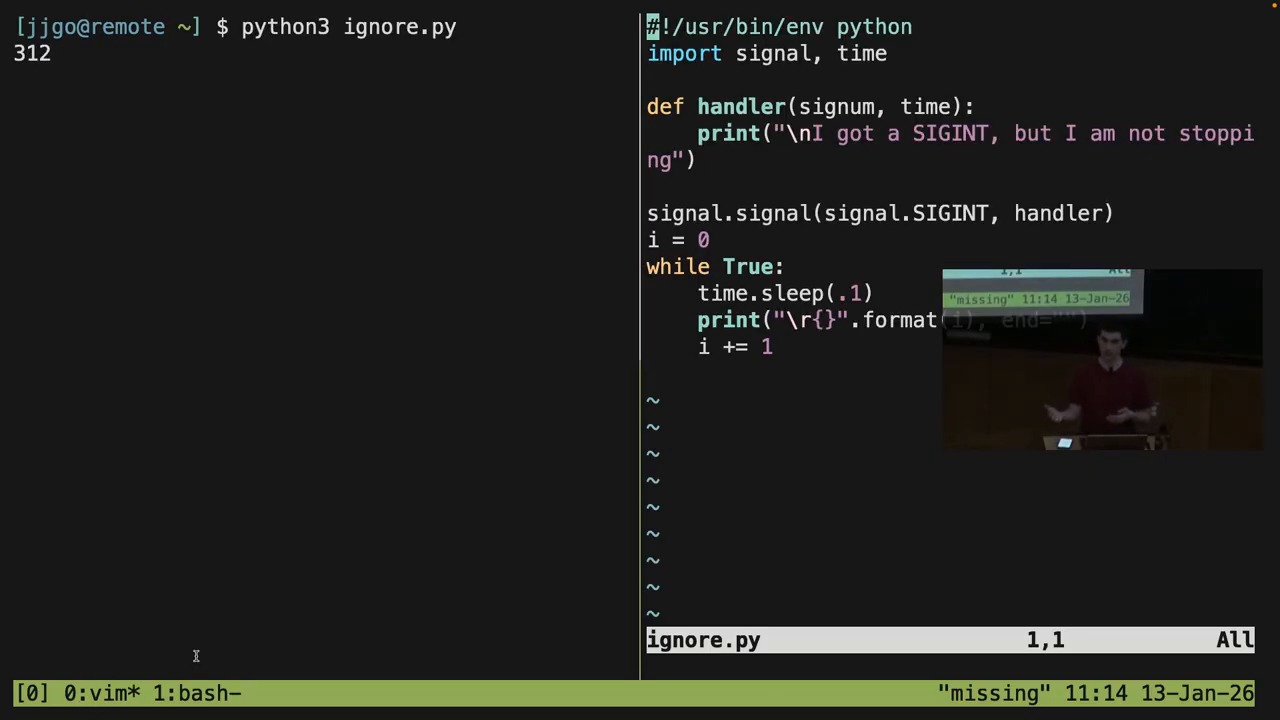
\includegraphics[width=0.92\textwidth]{figures/fig_20_tmux_panes.jpg}
\caption{在 tmux 中分出多个窗格，一边运行程序一边编辑文件\vtag}
\end{figure}
\srcnote{00:38:30--00:38:45}
\end{minipage}


把 Python 脚本拷到远程机器上运行后，问题来了：脚本一运行，这台远程机器上就什么也干不了了。这就是终端复用器的用武之地，最有名的是 tmux。终端复用器是让人方便地在同一个环境里运行许多程序的程序。运行 tmux 后，可以分出多个窗格（pane），比如一边让进程继续运行，一边在另一个窗格里编辑文件；还可以创建更多窗口（window），讲者说窗口是 tmux 的术语，可以把它想成浏览器的标签页，屏幕下方显示着编号 $0$ 和 $1$，可以在它们之间切换。

tmux 使用一种不太常见的快捷键：前缀式快捷键。通常总是先按 Ctrl+B，松开，再按另一个键。例如 Ctrl+B 再按 $0$，就跳到 $0$ 号窗口。讲义里列出了 tmux 的许多快捷键。

\noindent\begin{minipage}{\textwidth}
\begin{figure}[H]
\centering
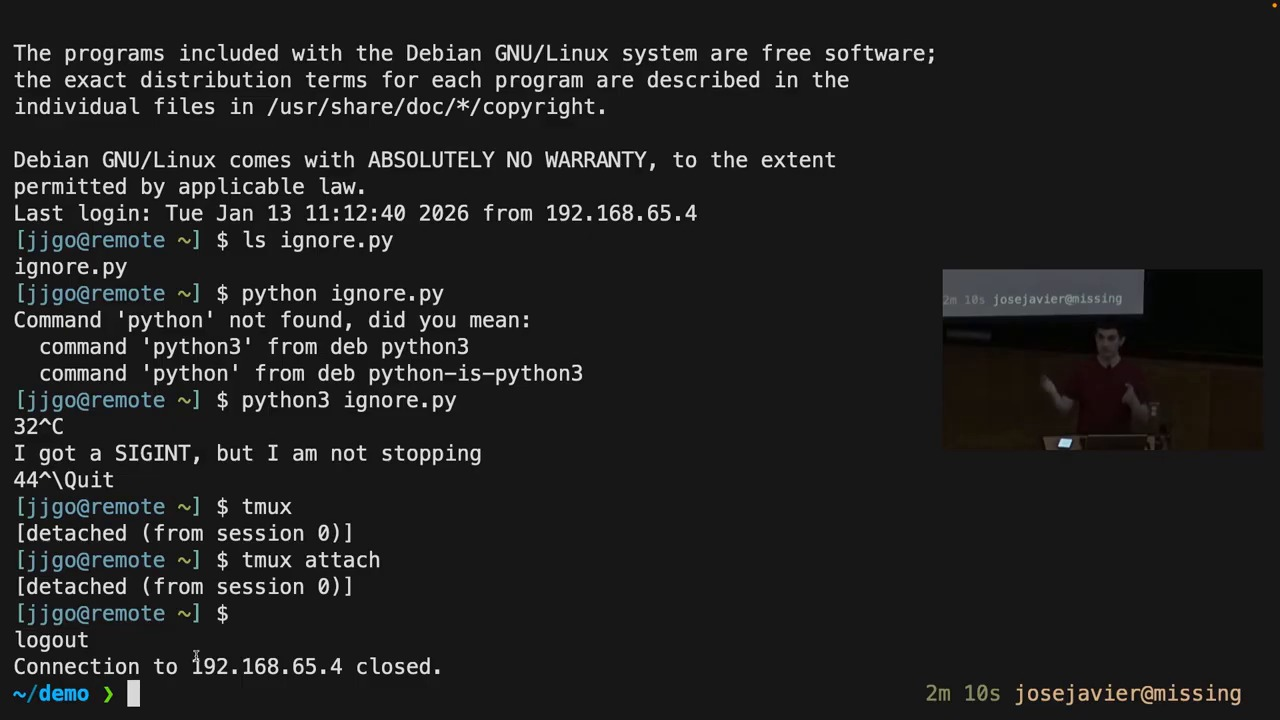
\includegraphics[width=0.92\textwidth]{figures/fig_21_tmux_detach.jpg}
\caption{从 tmux 会话分离后重新连接，程序仍在运行\vtag}
\end{figure}
\srcnote{00:39:45--00:40:00}
\end{minipage}


tmux 还能让整个会话保持运行：按 Ctrl+B 再按 D 分离（detach），之后可以重新连接（attach）。这样做的好处在于：如果程序直接运行在 SSH 会话里，一旦与远程服务器断开连接，程序就没了。因为断开远程会话时，Shell 会检测到这件事并发送一种特殊的信号，叫挂断信号 \texttt{SIGHUP}，它会杀死所有正在运行的进程。而 tmux 会接住这个信号，所以重新连接上去，会看到一切还在运行。讲者说这非常方便：远程会话不再与两台机器之间的连接绑在一起。

\begin{practicebox}{tmux 最常用的操作}
讲义作者整理（前缀为 Ctrl+B）：
\begin{itemize}
\item \texttt{tmux new -s name} 新建命名会话，\texttt{tmux ls} 列出会话，\texttt{tmux a -t name} 重新连接；
\item 前缀 + \texttt{d} 分离；前缀 + \texttt{c} 新建窗口，前缀 + 数字切换窗口；
\item 前缀 + \texttt{"} 和前缀 + \texttt{\%} 分别上下、左右切分窗格，前缀 + 方向键在窗格间移动。
\end{itemize}
\end{practicebox}

\subsection{本章小结}

tmux 在一个终端里提供多个窗口和窗格，更重要的是会话可以分离再连接，不受 SSH 断线时 \texttt{SIGHUP} 的影响。接下来回到自己的环境，看看怎样定制 Shell。

\section{定制 Shell}

\subsection{包管理器}

\noindent\begin{minipage}{\textwidth}
\begin{figure}[H]
\centering
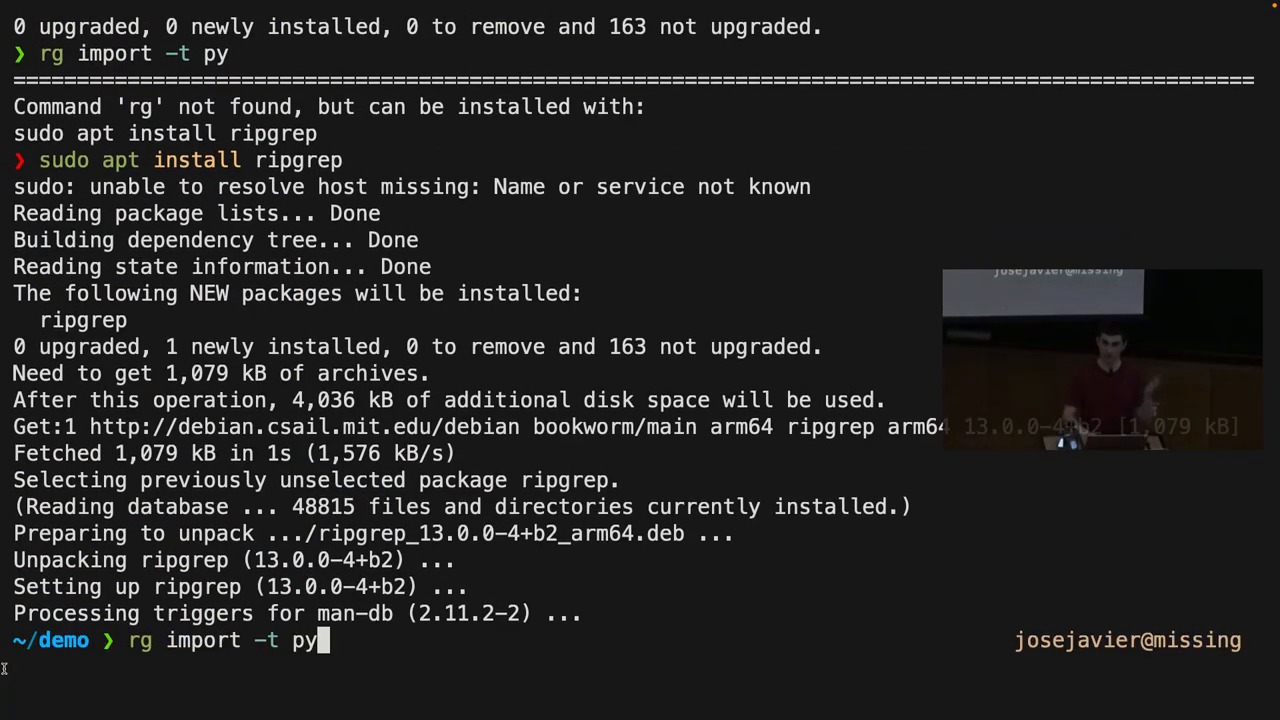
\includegraphics[width=0.92\textwidth]{figures/fig_22_ripgrep.jpg}
\caption{用 \texttt{apt} 安装 ripgrep 后，\texttt{rg} 命令才可用\vtag}
\end{figure}
\srcnote{00:43:00--00:43:15}
\end{minipage}


默认情况下，Shell 里只有操作系统自带的那些程序。比如照着课上的步骤运行 tmux，可能会发现它不存在，因为没有安装。安装程序通常用包管理器：在 macOS 上事实标准是 brew，在 Debian 和 Ubuntu 上是 APT，形如 \texttt{sudo apt install tmux}。

还有许多程序能让使用 Shell 更轻松。例如 ripgrep 是 \texttt{grep} 的更通用版本。讲者想找出所有包含 \texttt{import} 的 Python 文件，但 \texttt{rg} 还没装，Shell 提示应当安装 ripgrep；装好之后，之前不可用的程序就能用了。为什么命令叫 \texttt{rg} 而包叫 ripgrep，这种不一致有时让人沮丧。讲者推荐一个网站 Command Not Found：输入不知道怎么安装的程序名，它会告诉你在各种操作系统上如何安装。他说第一反应永远应该是先去包管理器里找。

\subsection{PATH 变量}

\noindent\begin{minipage}{\textwidth}
\begin{figure}[H]
\centering
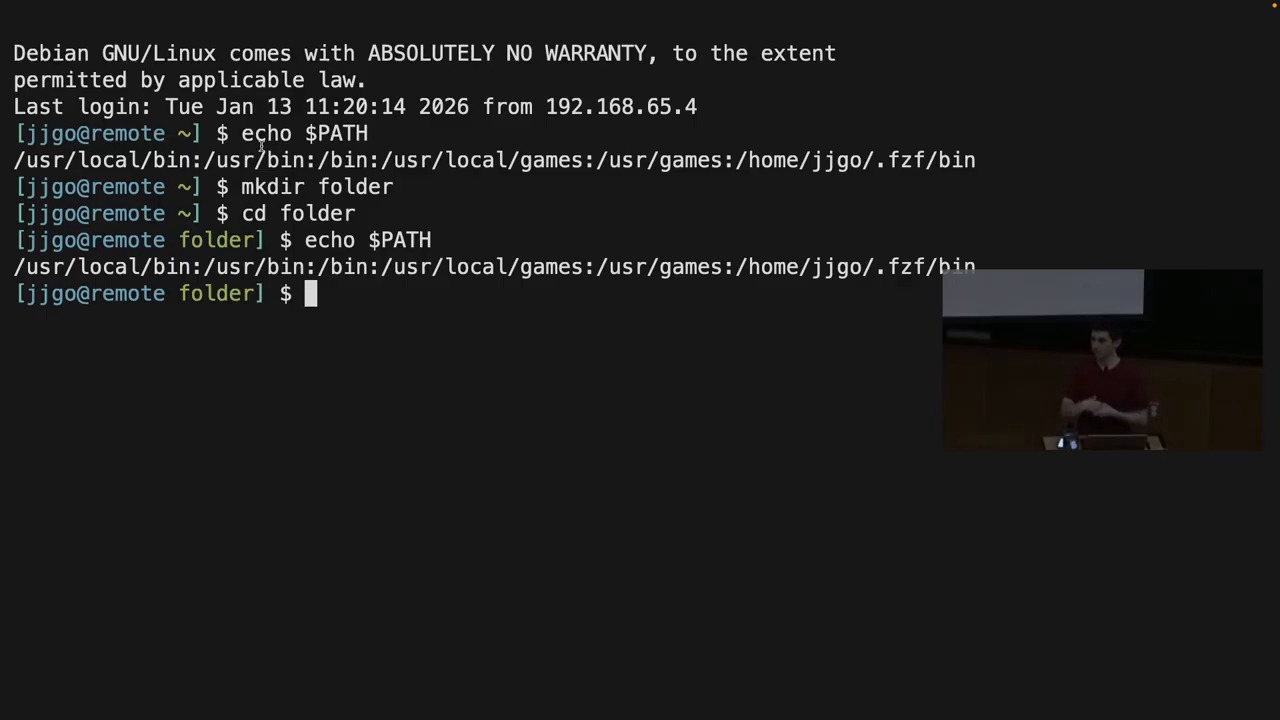
\includegraphics[width=0.92\textwidth]{figures/fig_23_path.jpg}
\caption{\texttt{PATH} 中列出的目录就是 Shell 寻找程序的地方\vtag}
\end{figure}
\srcnote{00:45:15--00:45:30}
\end{minipage}


\texttt{PATH} 环境变量包含一系列目录，Shell 在这些目录中寻找所有程序。根据前面学到的知识，修改 \texttt{PATH} 让它多一项，不过就是一次变量赋值：\texttt{PATH} 等于原来的值再加上要追加的新路径；而且大概应该 \texttt{export}，否则子进程不会继承它。

有同学问 \texttt{PATH} 是不是当前所在的位置。讲者说不是：\texttt{PATH} 是一个变量，进入一个新目录后它并没有变。默认情况下，Shell 不会在当前目录里找程序，这就是为什么上一讲运行自己写的脚本时要加 \texttt{./} 前缀。直接输入 \texttt{script.sh}，Shell 会说在这些目录里都找不到这个命令；执行 \texttt{export} 追加目录之后，\texttt{PATH} 多了一项，Shell 就会在那里查找。

\begin{lstlisting}[language=bash]
export PATH="$PATH:/path/to/append"
\end{lstlisting}

\subsection{让修改持久化}

\noindent\begin{minipage}{\textwidth}
\begin{figure}[H]
\centering
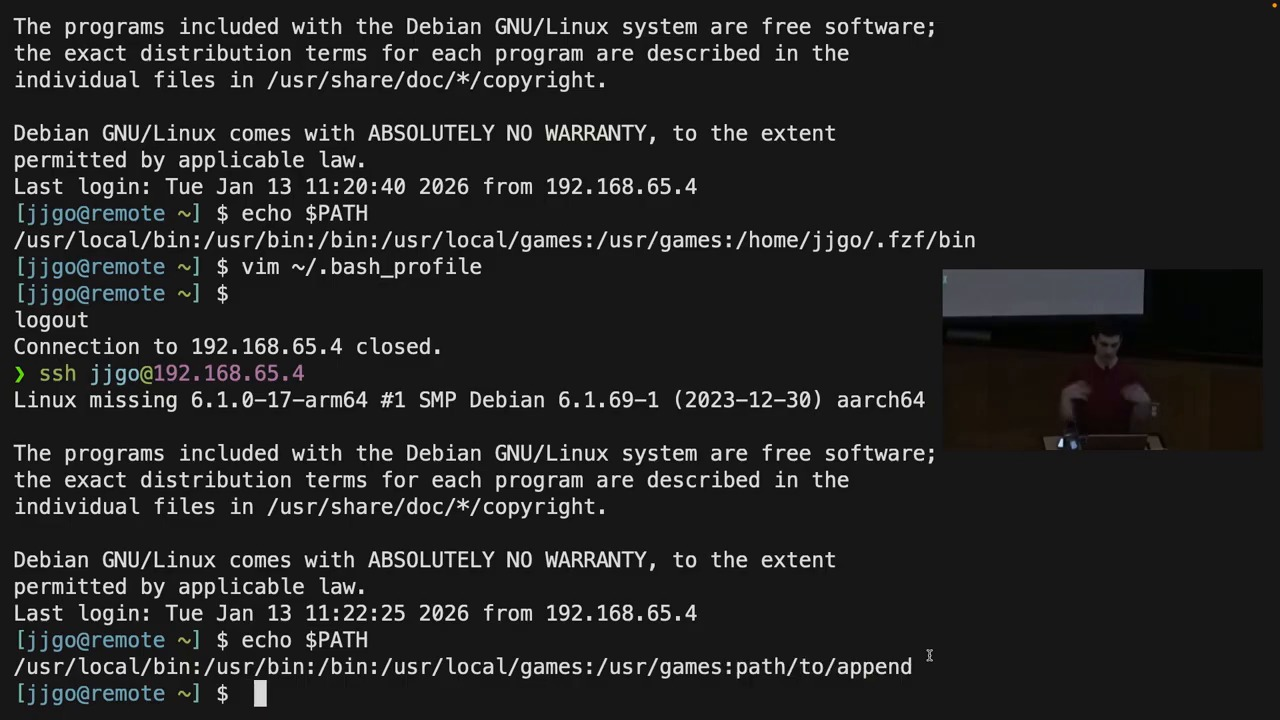
\includegraphics[width=0.92\textwidth]{figures/fig_24_bashrc.jpg}
\caption{把 \texttt{export PATH=...} 写进 \texttt{.bashrc}，并用 \texttt{PS1} 修改提示符\vtag}
\end{figure}
\srcnote{00:47:15--00:47:30}
\end{minipage}


问题是断开再重新连接、开启新会话后，再看 \texttt{PATH}，那项修改已经丢了：即使为子进程 \texttt{export} 了，它也没有被持久保存，新会话并不知道它。要持久化配置，就要把它加入 Shell 的配置文件，具体取决于运行的是哪个 Shell。远程服务器上运行的是 bash，配置文件是 \texttt{.bashrc} 或 \texttt{.bash\_profile}。Shell 启动时会读取这个文件，逐行执行，于是 \texttt{PATH} 就有了这一项。讲者断开再连接验证了这一点。

\texttt{PATH} 是一个特殊变量，还有些变量控制 Shell 行为的其他方面。例如 \texttt{PS1} 告诉 Shell 怎样渲染左侧的提示符：把它改成一个简单的符号，再启动一个新 Shell，提示符就只剩那个符号了。设置这类变量需要使用 Shell 能理解的特定语法。

\begin{knowledgebox}{\texttt{.bashrc} 与 \texttt{.bash\_profile}}
讲者说讲义里有一个很有用的链接，解释为什么会有多个配置文件、什么时候读哪一个。简单说，bash 区分登录 Shell 和交互式非登录 Shell：像课上这样的交互式会话会读 \texttt{.bashrc}，登录 Shell 读 \texttt{.bash\_profile}。zsh 则读取完全不同的文件，如 \texttt{.zshrc}，所以两个 Shell 可以完全独立地配置。讲义作者补充：常见做法是在 \texttt{.bash\_profile} 里 \texttt{source \textasciitilde/.bashrc}，把配置集中到一处。
\end{knowledgebox}

\subsection{覆盖 Shell 的行为：fzf}

\noindent\begin{minipage}{\textwidth}
\begin{figure}[H]
\centering
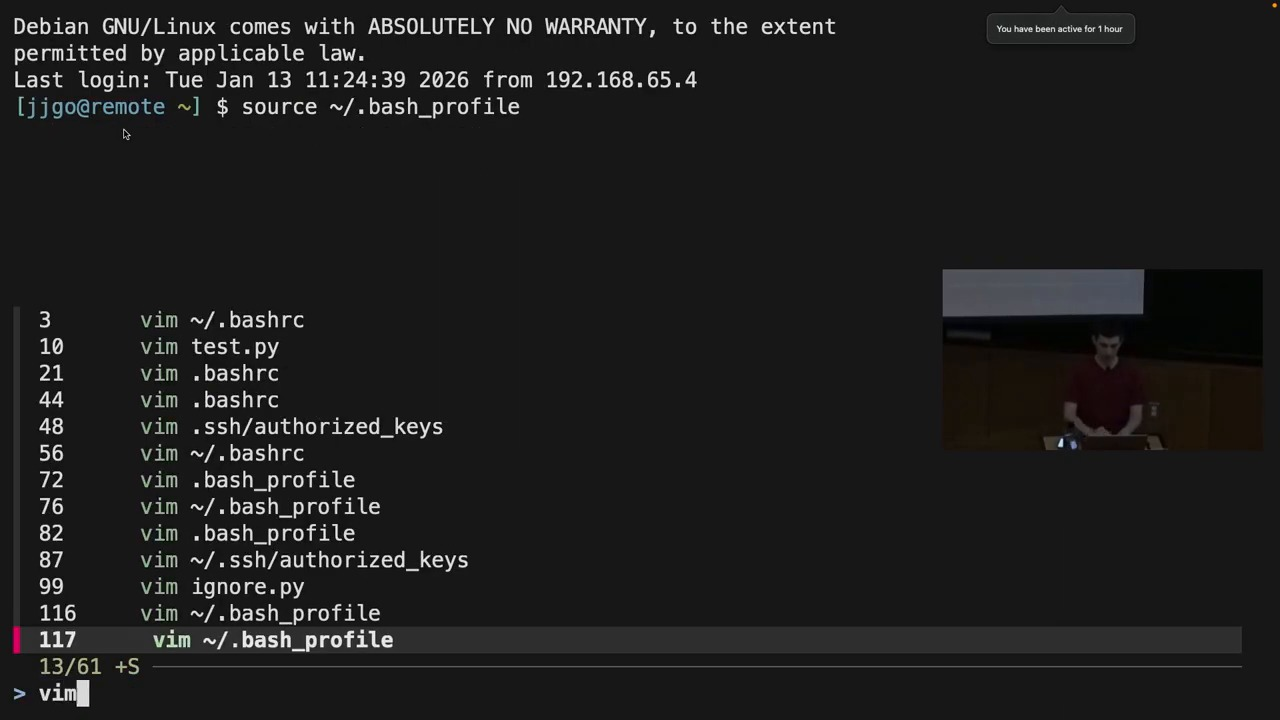
\includegraphics[width=0.92\textwidth]{figures/fig_25_fzf.jpg}
\caption{加载 fzf 后，Ctrl+R 变成对历史命令的模糊搜索\vtag}
\end{figure}
\srcnote{00:49:00--00:49:15}
\end{minipage}


找命令时可以利用历史记录：讲者知道自己某个时候运行过 vim 命令，可以用 Ctrl+R 在历史里向后搜索。Shell 也允许覆盖这种行为。这里加载另一个工具 fzf，一个模糊查找器（fuzzy finder），它挂接到 Shell 上，覆盖 Ctrl+R 的行为。不退出 Shell 就让配置生效的办法是 \texttt{source}，意思是逐行执行那个文件。现在按 Ctrl+R，就得到一个列出所有运行过的 vim 命令的模糊查找界面。

\subsection{dotfiles}

\noindent\begin{minipage}{\textwidth}
\begin{figure}[H]
\centering
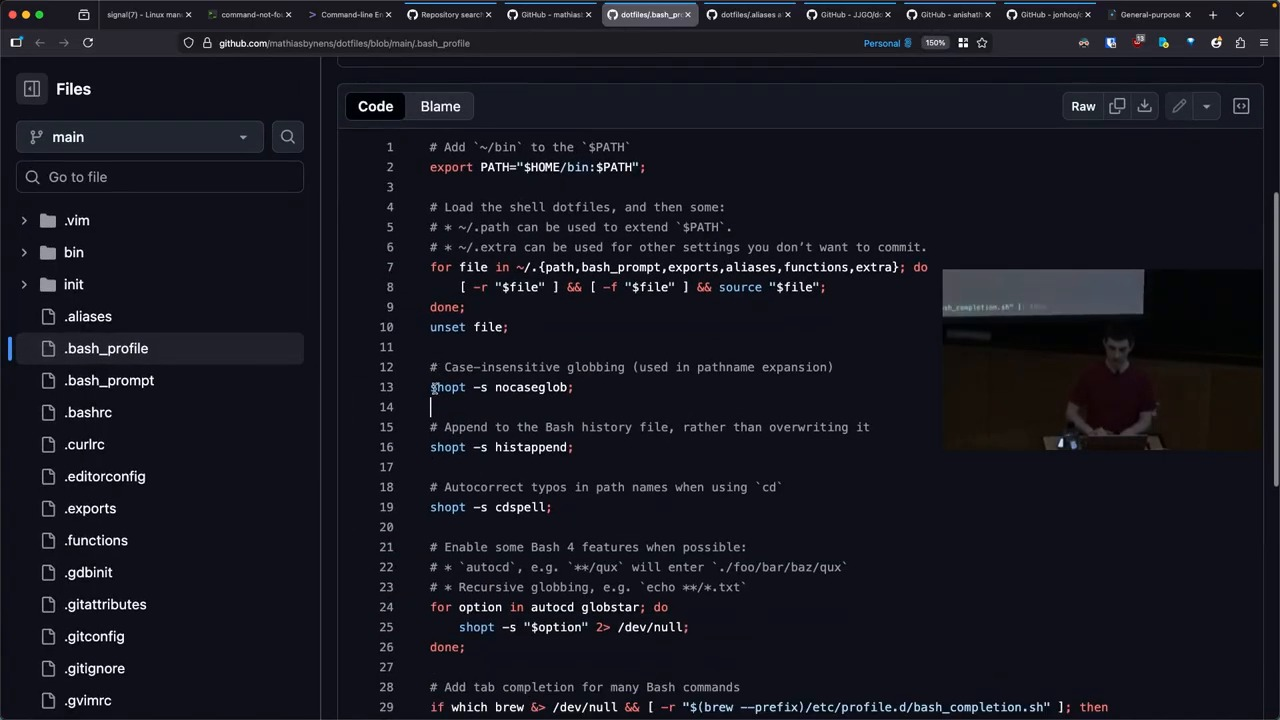
\includegraphics[width=0.92\textwidth]{figures/fig_26_dotfiles_github.jpg}
\caption{在 GitHub 上公开的他人 dotfiles 可以作为学习材料\vtag}
\end{figure}
\srcnote{00:50:00--00:50:15}
\end{minipage}


Shell 可以定制的东西非常多，还有完整的插件系统。很多人会把自己的环境配置记录在网上，这通常叫 dotfiles，因为这些文件大多以点开头而被隐藏，比如 \texttt{.bashrc}、\texttt{.zshrc}。讲者说阅读别人的 dotfiles 很有用：例如某个用户不希望通配符区分大小写，就用一个选项告诉 Shell 在匹配时不区分大小写，网上有人记录了大量这样的选项。

\noindent\begin{minipage}{\textwidth}
\begin{figure}[H]
\centering
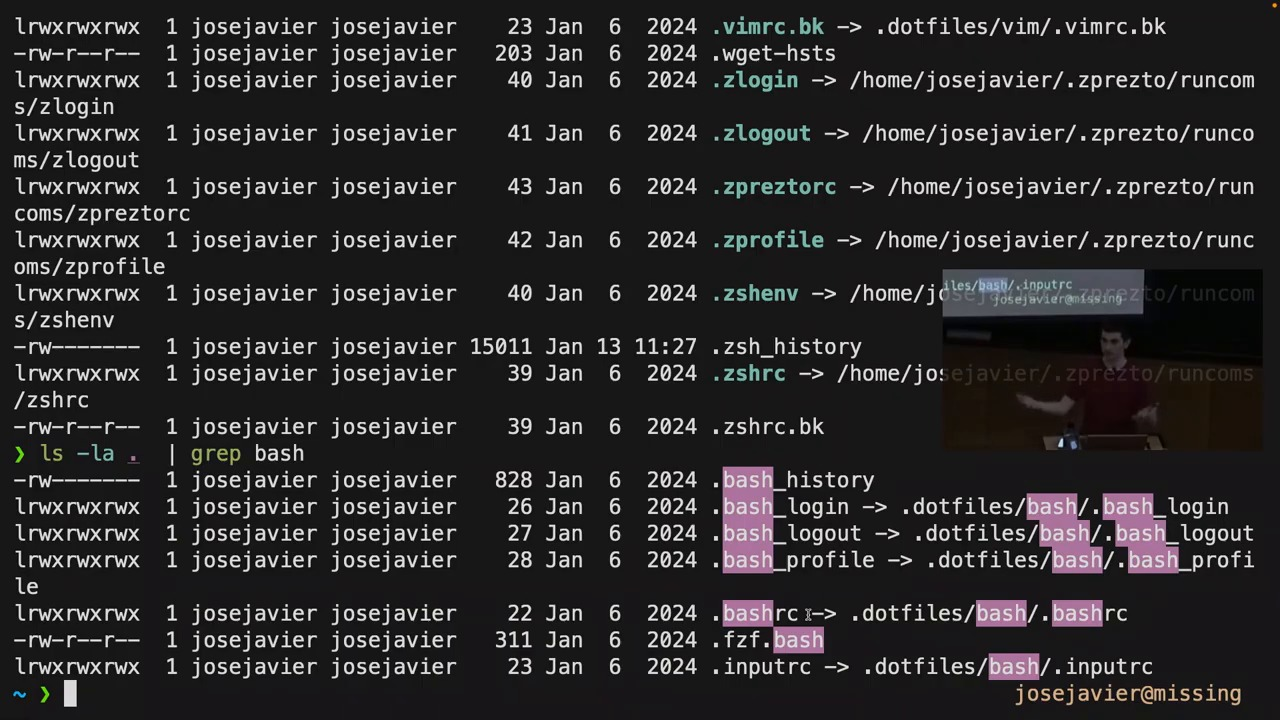
\includegraphics[width=0.92\textwidth]{figures/fig_27_symlinks.jpg}
\caption{\texttt{ls -la} 显示配置文件是指向 \texttt{\textasciitilde/.dotfiles} 中文件的符号链接\vtag}
\end{figure}
\srcnote{00:51:00--00:51:15}
\end{minipage}


还有一个细节：为了换到另一台机器时不丢失配置，值得把它们集中放在一个地方，再安装到当前环境。讲者用 \texttt{ls -la} 展示了符号链接：符号链接是许多操作系统里的概念，意思是“谁要读这个文件，就去读另一个文件”。例如读 \texttt{.bashrc} 时实际读的是 \texttt{.dotfiles/bash/bashrc}。这样他把所有 dotfiles 放在 \texttt{.dotfiles} 下做版本管理，放在 GitHub 上；配置新电脑时，只需运行一个创建这些符号链接的脚本，程序就能找到配置文件。

\begin{warningbox}{不要整份照抄别人的配置}
讲者建议不要不加理解地照抄别人的整个 \texttt{.bashrc}，那样会让人非常困惑；从默认状态出发，逐行理解要加的东西更有用。
\end{warningbox}

\subsection{插件}

\noindent\begin{minipage}{\textwidth}
\begin{figure}[H]
\centering
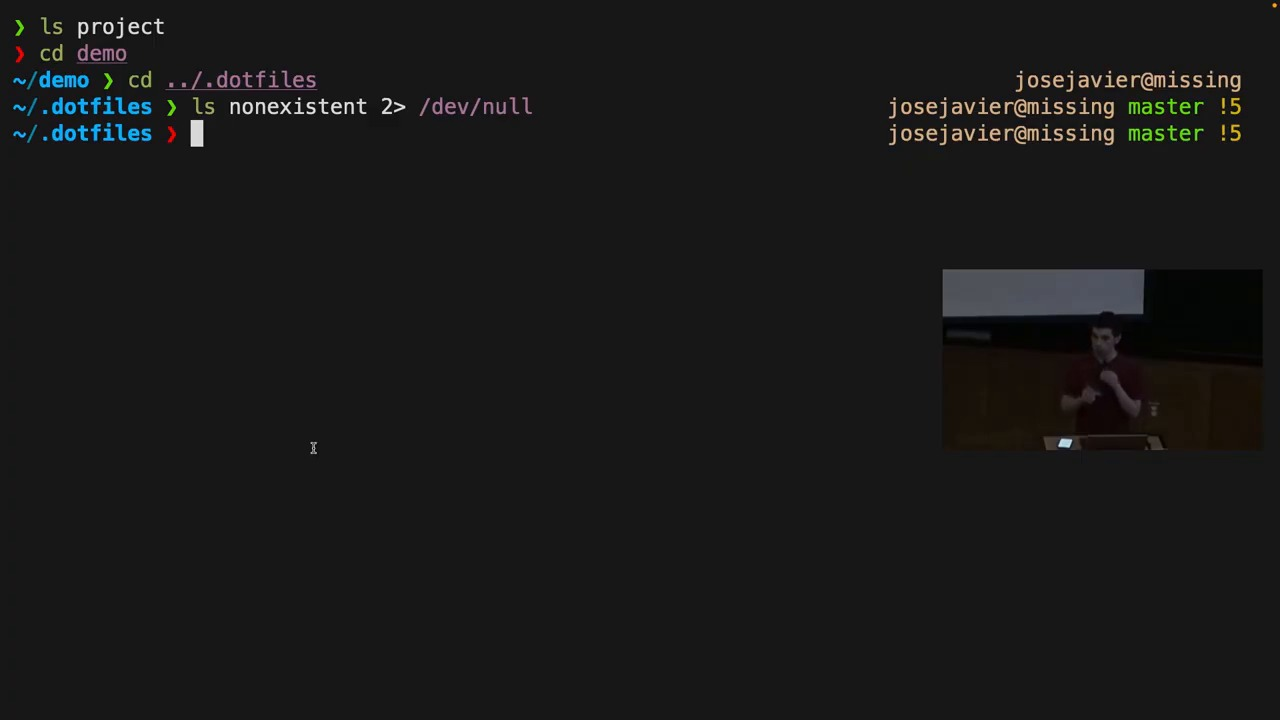
\includegraphics[width=0.92\textwidth]{figures/fig_28_zsh_plugins.jpg}
\caption{zsh 插件提供的语法高亮与包含 git 状态的提示符\vtag}
\end{figure}
\srcnote{00:56:00--00:56:15}
\end{minipage}


有些功能不是 Shell 内置的，但很方便，于是有人做成插件包。讲者的终端里，命令在输入时就会被着色：输入 \texttt{ls} 显示为绿色，因为这个命令存在；输入 \texttt{ls} 之外不存在的命令则是红色，甚至不必运行就知道它不可用。这是他让 zsh 加载了一些文件实现的，讲义里有这类插件的链接。

有些插件还会配置提示符的样子：提示符告诉他现在是哪台机器上的哪个用户；进入 dotfiles 目录时，会显示只与该目录相关的信息，例如在这个 git 仓库里处于 master 分支、有 $5$ 处改动尚未提交；如果运行了一个不存在的命令，光标会变红，因为上一个命令的返回码非零。讲者说这些信息手动也能拿到，只是这样一眼就能看到。

\noindent\begin{minipage}{\textwidth}
\begin{figure}[H]
\centering
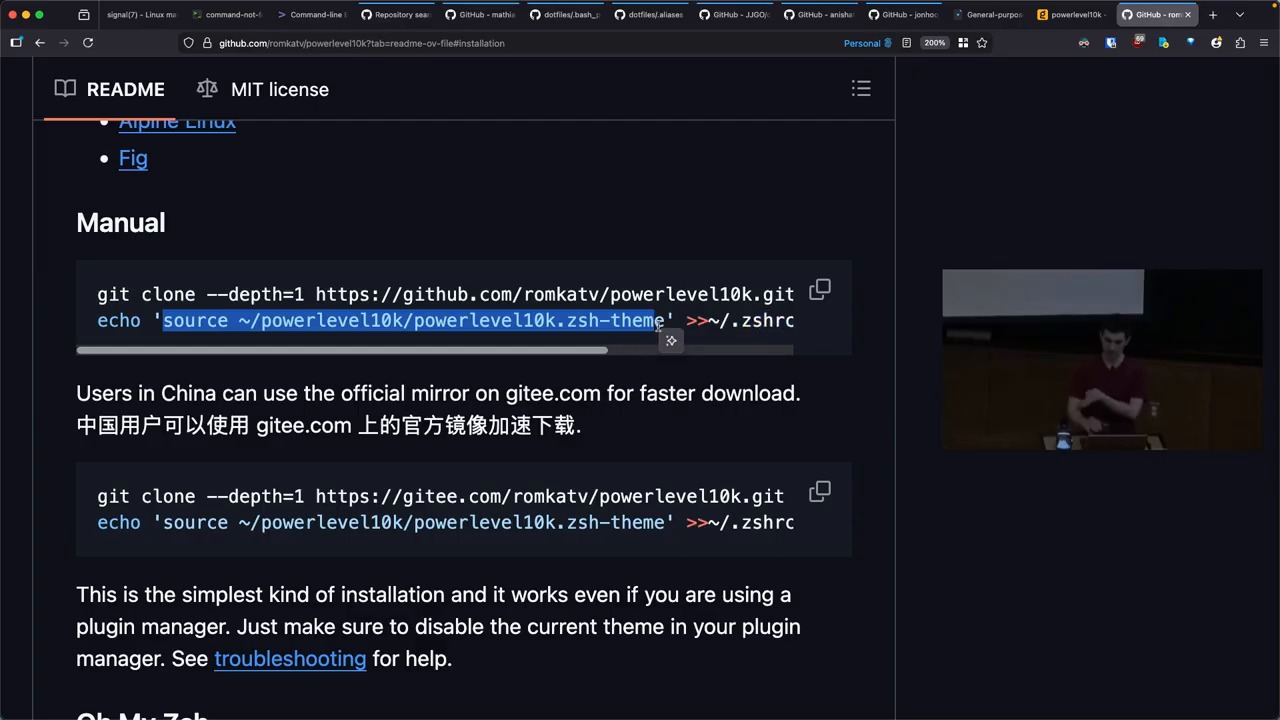
\includegraphics[width=0.92\textwidth]{figures/fig_29_plugin_install.jpg}
\caption{插件安装说明：\texttt{git clone} 仓库后在 \texttt{.zshrc} 中加入一行 \texttt{source}\vtag}
\end{figure}
\srcnote{00:59:15--00:59:30}
\end{minipage}


有同学问这在 WSL 里是否可用：可以，因为 WSL 大体上可以看作在你的电脑里运行的一台 Linux 机器。又问这会不会影响所有 Shell、所有目录：在目录之间切换时仍是同一个 Shell 会话，所以会；但如果从配置好的 zsh 里启动一个 bash，bash 用的是另一套配置。讲者说他特意没有修改 bash，把它留作出问题时的后备。

\noindent\begin{minipage}{\textwidth}
\begin{figure}[H]
\centering
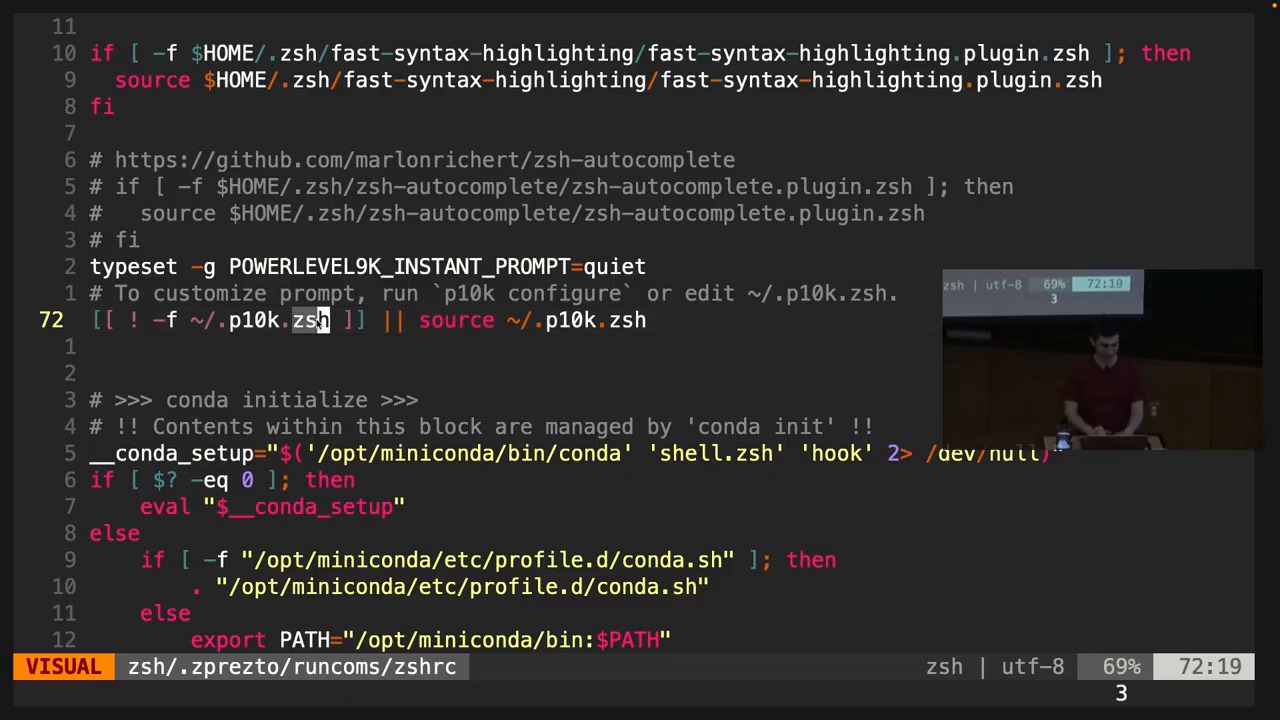
\includegraphics[width=0.92\textwidth]{figures/fig_30_zshrc.jpg}
\caption{\texttt{.zshrc} 中按条件 \texttt{source} 各个插件文件的几行配置\vtag}
\end{figure}
\srcnote{00:58:00--00:58:15}
\end{minipage}


讲者打开 \texttt{.zshrc} 展示了 powerlevel10k 提示符插件：那一行的意思是如果某个文件存在就 \texttt{source} 它，\texttt{source} 会逐行执行文件内容；那个文件本身是一个用 zsh 写的完整插件。插件通常托管在 GitHub 上，有安装说明，最简单的就是 \texttt{git clone} 把仓库下载到本机的某个路径，再加一行启用它。说明里的命令甚至直接把这行追加到 \texttt{.zshrc}，不必用 vim 手动编辑。

\begin{importantbox}{一次只装一个插件}
讲者提醒，有些框架会一次加载大量插件，它们可能不错，但也会拖慢 Shell，因为它们替你做了很多事。他建议一次只安装一个插件，看自己是否真的在用、是否值得，不值得就删掉。这种细粒度的控制能防止 Shell 变得臃肿。
\end{importantbox}

\subsection{本章小结}

用包管理器安装工具，用 \texttt{PATH} 决定去哪里找程序，把配置写进 \texttt{.bashrc} 或 \texttt{.zshrc} 才能持久，用 dotfiles 与符号链接在多台机器间同步配置，插件则按需逐个添加。最后看看 AI 工具怎样进入 Shell。

\section{Shell 中的 AI 与终端模拟器}

\subsection{命令生成}

\noindent\begin{minipage}{\textwidth}
\begin{figure}[H]
\centering
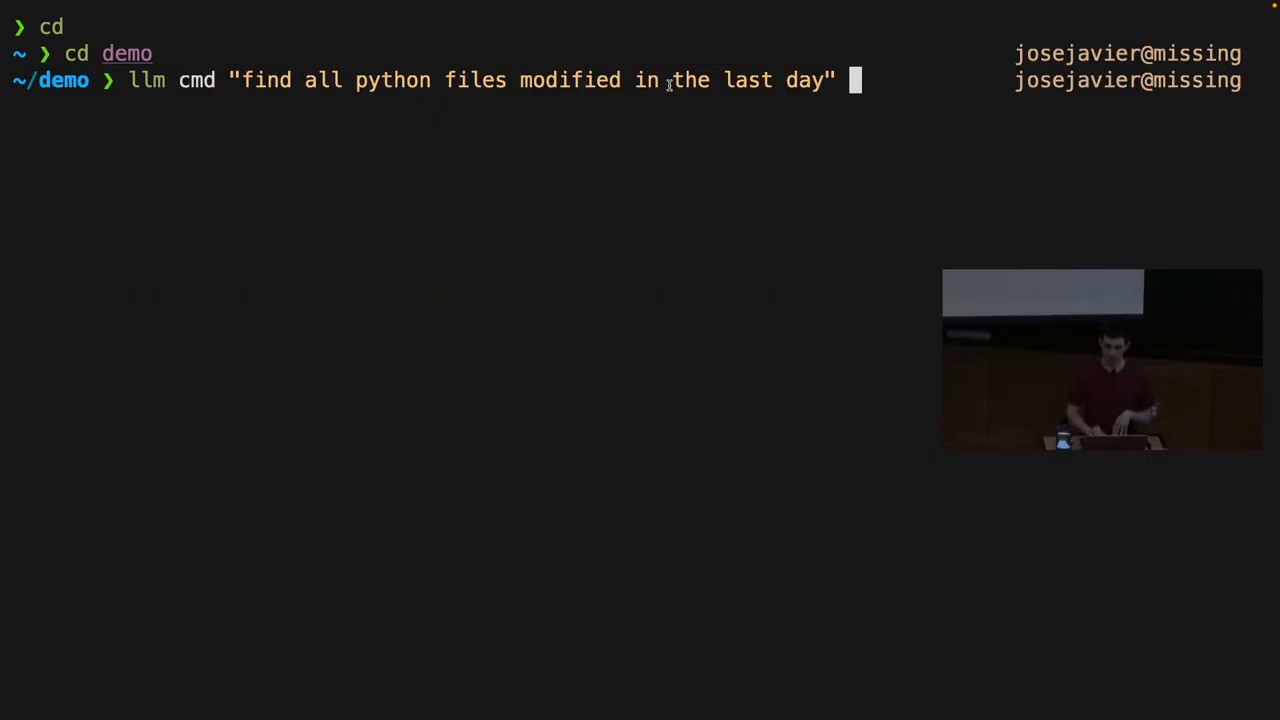
\includegraphics[width=0.92\textwidth]{figures/fig_31_llm_cmd.jpg}
\caption{\texttt{llm cmd} 根据自然语言描述生成 \texttt{find} 命令并询问是否执行\vtag}
\end{figure}
\srcnote{01:01:00--01:01:15}
\end{minipage}


讲者说，你当然可以打开 ChatGPT 的网页问它 Shell 的问题，而且一定有用，但也可以直接在 Shell 里与 AI 交互。他用的是 llm 这个工具：描述“我想要一个命令，找出最近一天修改过的所有 Python 文件”。他知道 \texttt{find} 有能做到这件事的语法，但正如上一讲 Jon 所说，\texttt{find} 的选项很难记全。LLM 很容易给出正确答案，并提示是否运行这条命令。快速检查一下，它在逻辑上说得通：名字匹配 \texttt{*.py}，必须是普通文件，必须是最近一天修改的。

\begin{lstlisting}[language=bash]
llm cmd "find all python files modified in the last day"
find . -name "*.py" -type f -mtime -1
\end{lstlisting}

\subsection{管道集成}

\noindent\begin{minipage}{\textwidth}
\begin{figure}[H]
\centering
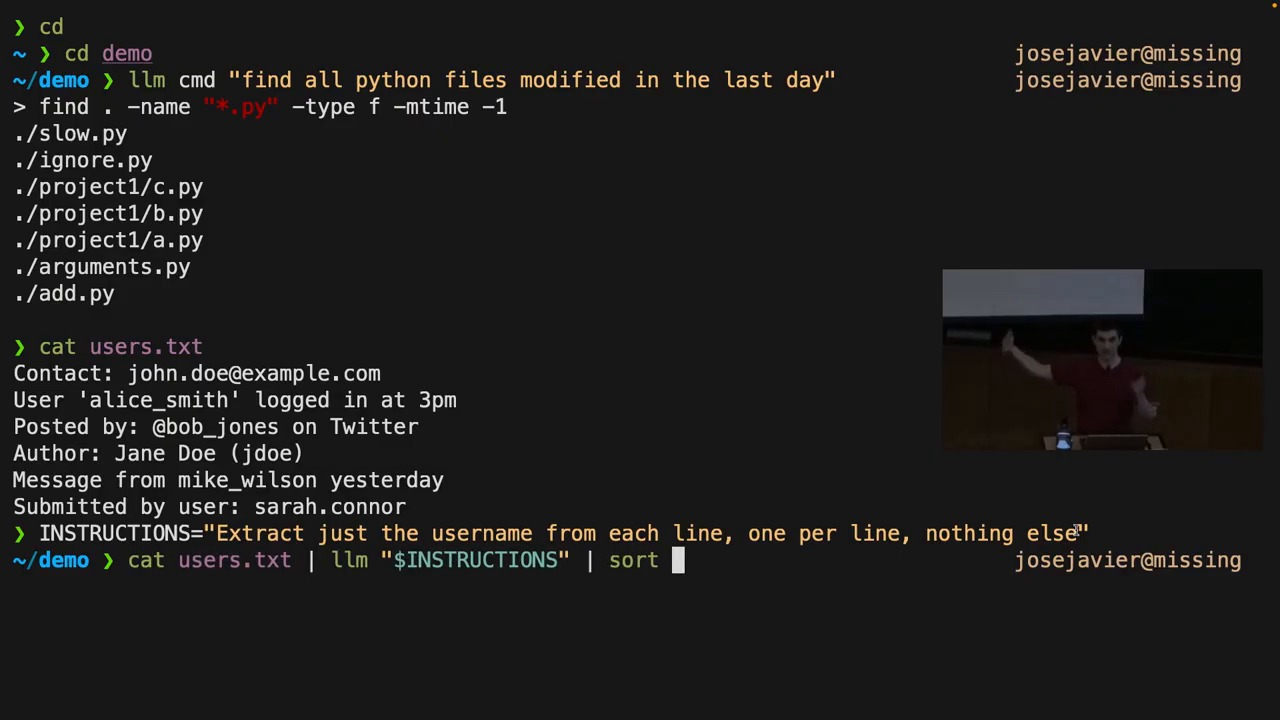
\includegraphics[width=0.92\textwidth]{figures/fig_32_llm_pipe.jpg}
\caption{把格式各异的文本经管道交给 LLM，按自然语言指令抽取用户名\vtag}
\end{figure}
\srcnote{01:02:15--01:02:30}
\end{minipage}


LLM 也可以嵌进管道，处理和转换数据。讲者展示了一个 \texttt{users.txt}，每行都提到一个用户名，但格式五花八门：邮件地址、引号里的名字、推特账号、括号里的缩写等。他说肯定存在一个能把它们都抽出来的正则表达式，但定义一个变量写上“只给我这一行的用户名，别的都不要”要简单得多，再把它交给 LLM。这也是一个好例子：LLM 程序通过参数拿到指令，通过管道拿到输入，输出再交给 \texttt{sort}。可以看到它为每一行抽出了相关信息，而用非结构化的解析来做会相当困难。

\begin{lstlisting}[language=bash]
INSTRUCTIONS="Extract just the username from each line, one per line, nothing else"
llm "$INSTRUCTIONS" < users.txt | sort
\end{lstlisting}

\subsection{AI Shell}

\noindent\begin{minipage}{\textwidth}
\begin{figure}[H]
\centering
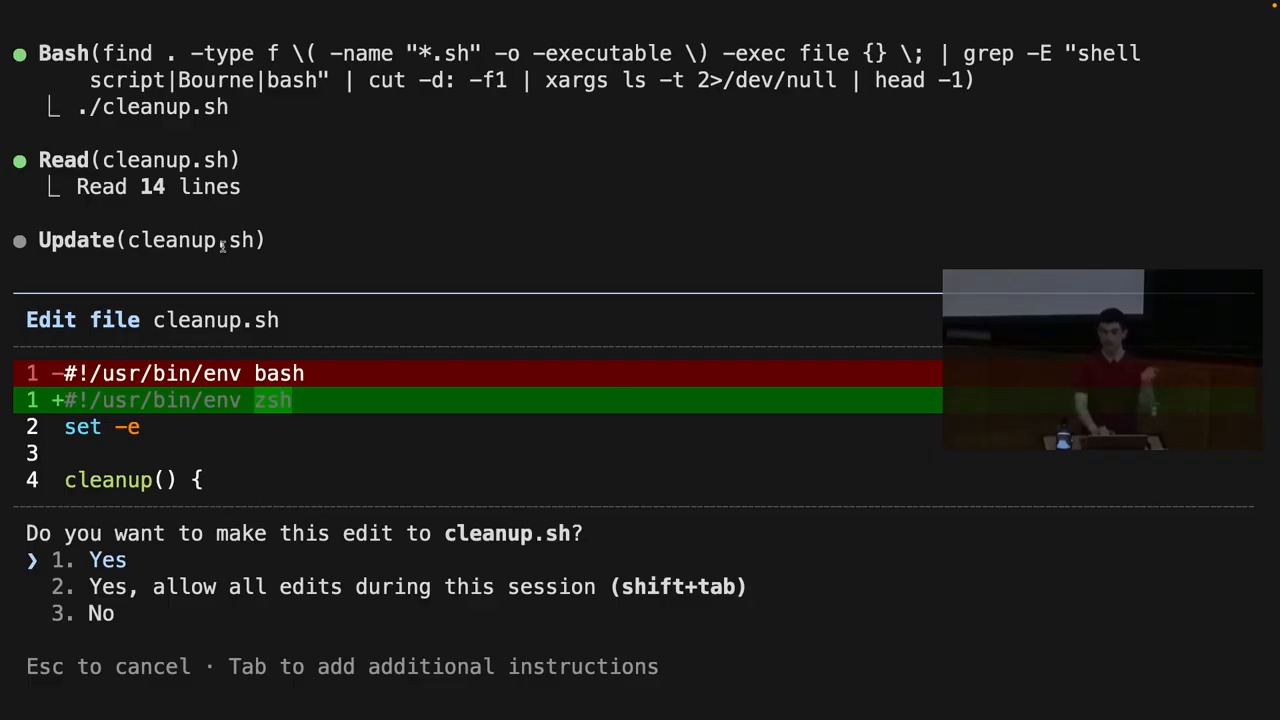
\includegraphics[width=0.92\textwidth]{figures/fig_33_claude_code.jpg}
\caption{Claude Code 把英文指令翻译成一条复杂的 \texttt{find} 管道并修改 shebang 行\vtag}
\end{figure}
\srcnote{01:04:15--01:04:30}
\end{minipage}


最后一个工具是 Claude Code，它更进一步：用英文给出指令，它会把其中许多转换成 Shell 操作。讲者说可以把它看作一个“元 Shell”程序，只不过编程语言是英语。他让它“再用 find 找出最近修改的 Shell 脚本，然后把 shebang 行改成用 csh”。这件事自己大概也能做，但 \texttt{find} 的语法很棘手；LLM 读取指令，生成了一条看起来非常陌生、充满不明所以之处的 bash 命令，但拆开来看完全合理：它搜索可执行的 \texttt{.sh} 文件，并找出其中最近修改的那个。运行后，它不需要我们拿着前一个命令的输出去琢磨怎样喂给下一个命令，而是确定了最近修改的是 \texttt{cleanup.sh}，并提出把 shebang 从 bash 改成 csh，我们可以接受这个修改。

\begin{warningbox}{先读懂再执行}
讲者每次都先检查 LLM 生成的命令再运行。讲义作者提醒：生成的命令可能删改文件，执行前至少确认它作用在哪些文件上、是否有破坏性的选项；对 \texttt{rm}、\texttt{mv}、\texttt{sed -i} 这类命令尤其如此。
\end{warningbox}

\subsection{终端模拟器}

\noindent\begin{minipage}{\textwidth}
\begin{figure}[H]
\centering
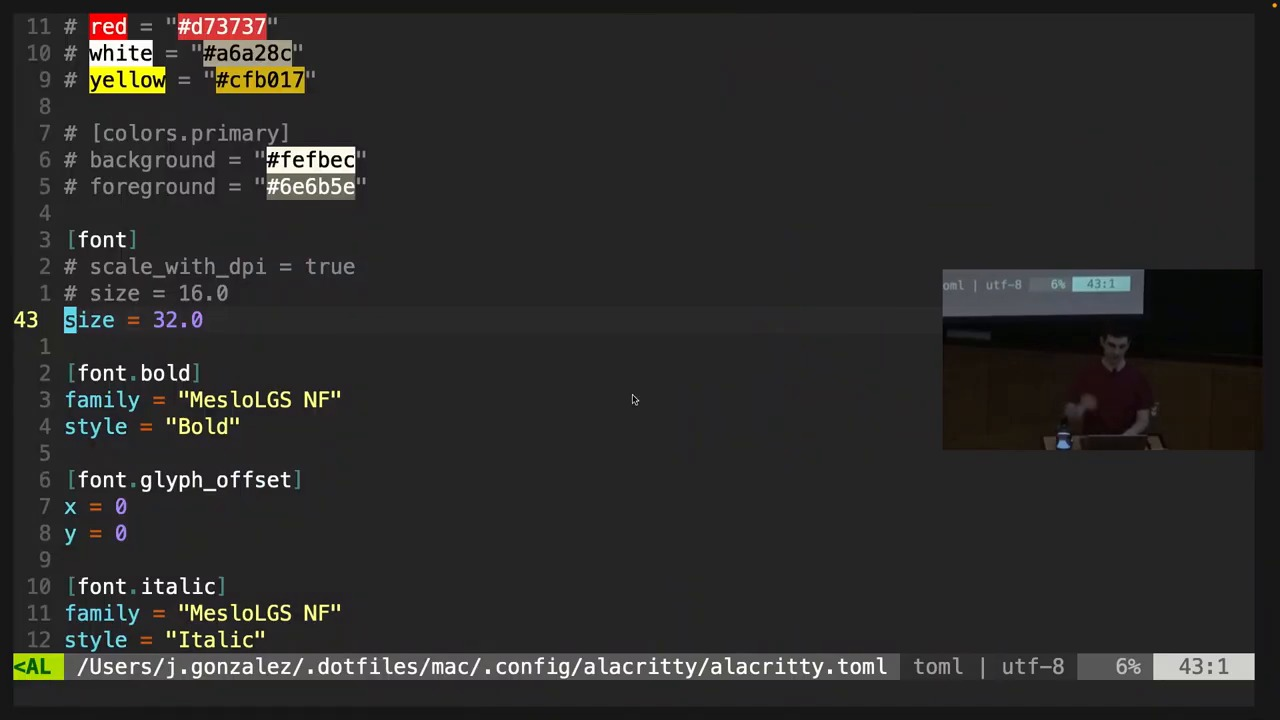
\includegraphics[width=0.92\textwidth]{figures/fig_34_terminal_emulator.jpg}
\caption{Alacritty 的配置文件 \texttt{alacritty.toml}，课上把字号设成了 32\vtag}
\end{figure}
\srcnote{01:05:30--01:05:45}
\end{minipage}


最后一件事：到目前为止，Shell 都运行在某个程序里，这取决于操作系统。这里用的是终端模拟器（terminal emulator），它是一个运行 Shell 并把它呈现在电脑上的图形界面程序。选择很多，和 dotfiles 一样值得研究用哪一个。讲者用的是 Alacritty，它也有可以配置的选项：例如为了这次讲课，他把字号从 $16$ 改成了 $32$，改回去就恢复成平时的大小。讲义提到，值得调整的方面包括字体、配色、快捷键、标签页与分屏、回滚缓冲区，以及性能，一些较新的终端如 Alacritty 和 Ghostty 支持 GPU 加速。

\subsection{本章小结}

AI 工具可以在三个层次进入 Shell：生成单条命令、作为管道中的一个处理环节、以及作为接受自然语言的“元 Shell”；无论哪种，执行前都要读懂命令。而承载这一切的终端模拟器，也值得像 dotfiles 一样认真配置。

\section{总结}

讲者以终端模拟器结束了这一讲，并在课后回答了个别问题。回顾全讲：
\begin{itemize}
\item 程序的输入是参数、标准输入和环境变量，输出是标准输出、标准错误和返回码，运行中还会收到信号；
\item 选项、短选项合并、\texttt{-} 表示标准输入、接受任意多个参数，都是程序之间的约定；通配符由 Shell 展开；
\item 管道中的程序并行运行；\texttt{export} 决定变量是否传给子进程；\texttt{\&\&}、\texttt{||} 和控制流依据返回码；
\item SSH 与密钥让我们在远程机器上工作，tmux 让会话不怕断线；
\item 包管理器、\texttt{PATH}、配置文件、dotfiles 和插件构成了可定制、可迁移的 Shell 环境；
\item AI 工具可以生成命令、处理管道数据，甚至直接执行多步任务，但执行前要先检查。
\end{itemize}

\begin{practicebox}{自测}
\begin{enumerate}
\item 运行 \texttt{touch -{}- -myfile}，再在不使用 \texttt{-{}-} 的情况下删掉它。
\item 解释 \texttt{foo = bar} 为什么不能定义变量，并说明 \texttt{DEBUG=1 cmd} 与 \texttt{export DEBUG=1} 的区别。
\item 用 \texttt{diff <(printenv | sort) <(export | sort)} 比较两者的输出，它们为什么不一样？
\item 写一个脚本，收到 \texttt{SIGINT} 时删除自己创建的临时文件。
\item 在远程机器上启动 tmux，运行一个长任务，分离、断开 SSH、重新连接后确认任务仍在运行。
\end{enumerate}
\end{practicebox}

\end{document}
